%% V1.3
%% 08/5/2018
%% by David McKnight

%% Initial skeletal IEEE LaTeX file obtained from Michael Shell's at http://www.michaelshell.org/

\documentclass[journal]{IEEEtran}
\usepackage{blindtext}
\usepackage{graphicx}
\usepackage{circuitikz}
\usepackage{tikz}
\usepackage{caption}
\usetikzlibrary{math} %needed tikz library
\usepackage{amsmath}
\usepackage{amssymb}
\usepackage{setspace}
\usepackage{svg}
\usepackage{commath}
\usepackage{mathtools}
\usepackage[super]{nth}


\newcommand{\mathsym}[1]{{}}
\newcommand{\unicode}[1]{{}}


\usepackage{mathrsfs}


\usepackage{float}
\usepackage{smartdiagram}
\usesmartdiagramlibrary{additions}

\usepackage[separate-uncertainty=true]{siunitx}

\DeclareCaptionType{equ}[][]
\captionsetup[equ]{justification=raggedleft, singlelinecheck=false, labelformat=empty}


% correct bad hyphenation here
\hyphenation{op-tical net-works semi-conduc-tor}

\begin{document}

% can use linebreaks \\ within to get better formatting as desired
\title{Signals and Systems Final Project}

\author{David~McKnight}

% The paper headers
\markboth{Signals~and~Systems,~Spring~2018, 4~May}%
{}
% The only time the second header will appear is for the odd numbered pages
% after the title page when using the twoside option.
% 
% *** Note that you probably will NOT want to include the author's ***
% *** name in the headers of peer review papers.                   ***
% You can use \ifCLASSOPTIONpeerreview for conditional compilation here if
% you desire.

% make the title area
\maketitle

\begin{abstract}
In this paper, we discuss the workings of the process of amplitude modulation (AM) and the associated technique of amplitude demodulation. Specifically, we examine how AM is used for transferring signal information over distances, and we develop and implement a system for retrieving modulated data at various frequencies from a collection of such signals through demodulation.
\end{abstract}
% IEEEtran.cls defaults to using nonbold math in the Abstract.
% This preserves the distinction between vectors and scalars. However,
% if the journal you are submitting to favors bold math in the abstract,
% then you can use LaTeX's standard command \boldmath at the very start
% of the abstract to achieve this. Many IEEE journals frown on math
% in the abstract anyway.


\section{Introduction}
A great deal of data can be conveyed in the form of a signal, and as transferal of data is useful, so, too, is the ability to transfer signals. For example, audio information can be converted into electromagnetic waves for transmittance from one place to another. Unfortunately, however, some waves propagate poorly, and it can be difficult to distinguish a signal from background noise, such as other transmittances. To rectify this, we can \textit{modulate} signals onto \textit{carrier signals}; in other words, we can attach our signal conveying information to a signal of a frequency less likely to be confused with other signals and that can be sent long distances. This, of course, necessitates that we be able to \textit{demodulate} the signal; that is, extract the original signal from the modulated version. In this paper, we explore the workings of modulation and demodulation and set up a system to perform demodulation of a sample containing \textit{amplitude modulated} (AM) waves containing voice clips of each of the NATO phonetic alphabet letters modulated on carrier waves ranging from \SI{20}{\kilo\hertz} through \SI{132.5}{\kilo\hertz} at \SI{4.5}{\kilo\hertz} intervals. We determine a system to demodulate the sample at each of these frequencies and implement the system with MATLAB. Finally, we play back the demodulated clips to determine onto carrier waves of which frequency each NATO phonetic letter was modulated.  

\section{Background}
Transmission of information has been important for a very long time, demonstrated, i.e., as far back as around 1800 ad with the US postal system to as far back as the hundreds BC with the Great Wall of China's beacon towers. More recently, however, we have been able to encode information representable as sums of sinusoids into more long-range signals. In the early 1900s, Reginald Fessenden implemented \cite{grant} a rudimentary version of what we refer to today as Amplitude Modulation, and others followed suit; however, progress for practical usage was stalled until signals could be sufficiently amplified prior to transmission. By the early 1920s, though, the technology started seeing practical use \cite{white}; since then, it has been used in many applications, including radio broadcasting, QAM, and two-way radios.

\section{Methods}
\subsection{Modulation}
The process of amplitude modulation consists of modulating a carrier wave by an offset version of the original signal; that is, multiplying the carrier wave by an offset version of our signal. Intuitively, we can imagine that if we have an original signal (represented by a sum of sinusoids) ranging in amplitude from some constant $a_1$ to some constant $a_2$, the amplitude of our (unit-magnitude) carrier wave, if multiplied by the original signal, will have its peak amplitude magnitudes scale from $a_1$ to $a_2$, and its overall amplitude shall vary with the original signal's. Such a signal is then transmitted wirelessly and decoded at some reception point. For example, consider the signal $f(x)=sin(x)+sin(2x)$ and the carrier wave $c(x)=sin(50x)$. If we multiply $g(x)$ by $h(x)=f(x)+d$, where $d$ brings $f(x)$ above the $\omega$-axis (in this case, $d\approx1.76017$), we have the equation as in eq. \eqref{fig:modulationsampletime}.

\begin{equation}
\begin{split}
h\left(x\right)c\left(x\right)&=\left(\sin{\left(x\right)}+\sin{\left(2x\right)}+1.76017\right)\sin{\left(50x\right)}\\
    &=1.76017\sin{\left(50x\right)} \\
    &+\frac{1}{2}\left(\cos{\left(48x\right)}+\cos{\left(49x\right)}\right)\\
    &-\frac{1}{2}\left(\cos{\left(51x\right)}-\cos{\left(52x\right)}\right)
\end{split}
\label{modulatedsignal}  
\end{equation}

\begin{figure}
    \centering
    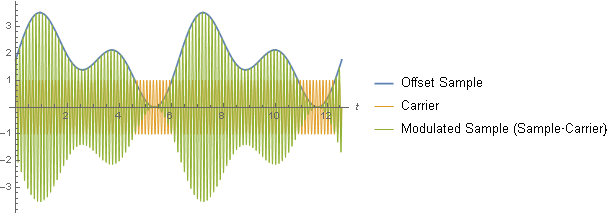
\includegraphics[width=\columnwidth]{ExampleV3TimeLong.png}
    \caption{The sample $\cos(t)+\cos(2t)$ modulated with the carrier $\cos(50t)$}
    \label{fig:modulationsampletime}
\end{figure}

If we shift to the frequency domain (although this is also evident from the time-domain equation), we recognize that magnitude responses of the original function are preserved, peaking about the carrier frequency rather than just the origin. For our example, this corresponds to peaks at $\SI{50\pm {1}}{rad\per\sec}$ and $\SI{50\pm{2}}{rad\per\sec}$, along with the carrier frequency peak of $\SI{50}{rad\per\sec}$, as seen in Fig. \ref{fig:modulationsamplefreq}. More generally, for each frequency $\omega_i$ of the sinusoids in the original sample, we now have, along with the carrier peak at $\omega_c$, peaks at $\omega_c+\omega_i$ and $\omega_c-\omega_i$. We now have a wave centered around the carrier frequency, and can transmit it to some other location. 

\begin{figure}[!hbt]
    \centering
    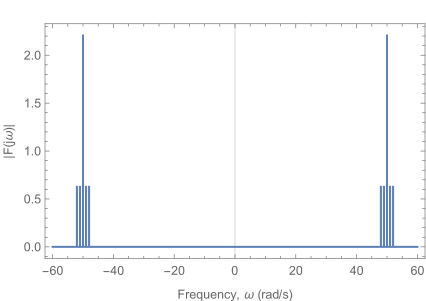
\includegraphics[width=\columnwidth]{ExampleV3Freq.png}
    \caption{The magnitude response of the sample $\cos(t)+\cos(2t)$ modulated with the carrier $\cos(50t)$}
    \label{fig:modulationsamplefreq}
\end{figure}

Once this has been done and the signal has been received, however, we require the ability to \textit{demodulate} the signal; that is, retrieve the original sinusoids of our sample. To do so, we need to bring our frequencies to the center.



\subsection{Demodulation}
\subsubsection{Demodulation Overview}
For demodulation, we need to undo modulation; that is, we need to take the offset frequencies from the modulated signal, center them at $\SI{0}{\hertz}$, and eliminate instances of the carrier frequency. 


\subsubsection{Pre-Demodulation Modulation}
For the purposes of explanation, we will use a modulated signal eq. \eqref{modulated} formed by modulating the sample signal given by eq. \eqref{sample} and the carrier signal given by eq. \eqref{carrier}.

\begin{equ}[ht]
    \begin{equation}
     s\left(t\right) = \cos{\left(10\cdot{}2\pi t\right)}+\cos{\left(25\cdot{}2\pi t\right)}
     \label{sample}
    \end{equation}
    \caption{Sample signal}
\end{equ}

\begin{equ}[ht]
    \begin{equation}
     c\left(t\right) = \cos{\left(1000\cdot{}2\pi t\right)}
     \label{carrier}
    \end{equation}
    \caption{Carrier signal}
\end{equ}

\begin{equ}[ht]
    \begin{equation}
    \begin{split}
    m\left(t\right)&=\left(\cos{\left(10\cdot{}2\pi t\right)}+\cos{\left(25\cdot{}2\pi t\right)}+2\right)\\
        &\cdot{}\cos{\left(1000\cdot{}2\pi t\right)}\\
        &=2\cos{(1000\cdot{}2\pi t)}\\
        &+\frac{1}{2}\left(\cos{\left(925\cdot{}2\pi t\right)}+\cos{\left(990\cdot{}2\pi t\right)}\right)\\
        &+\frac{1}{2}\left(\cos{\left(1010\cdot{}2\pi t\right)}+\cos{\left(1025\cdot{}2\pi t\right)}\right)
    \end{split}
    \label{modulated}
    \end{equation}
    \caption{Modulated signal}
\end{equ}

A time plot of a period of and a plot of the magnitude response for our sample are given by Fig. \ref{SampleTime} and Fig. \ref{SampleMagResponse}, respectively. 

\begin{figure}[ht]
	\centering
    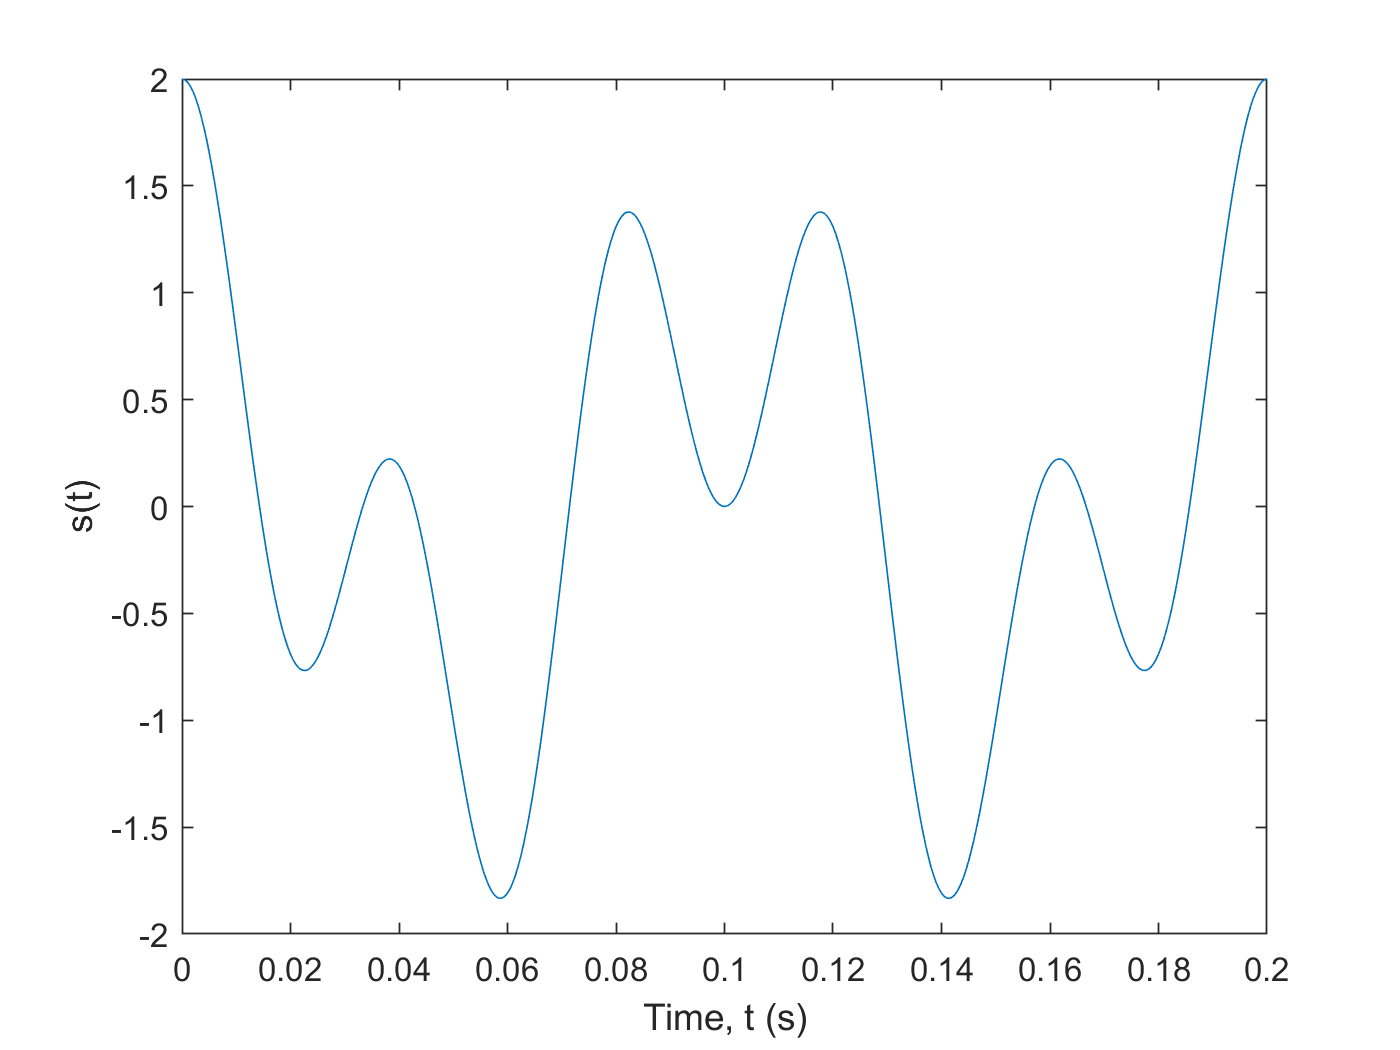
\includegraphics[width=\columnwidth]{SampleTime.png}
    \caption{One period of our sample signal, $s(t)$}
    \label{SampleTime}
\end{figure}

\begin{figure}[ht]
	\centering
    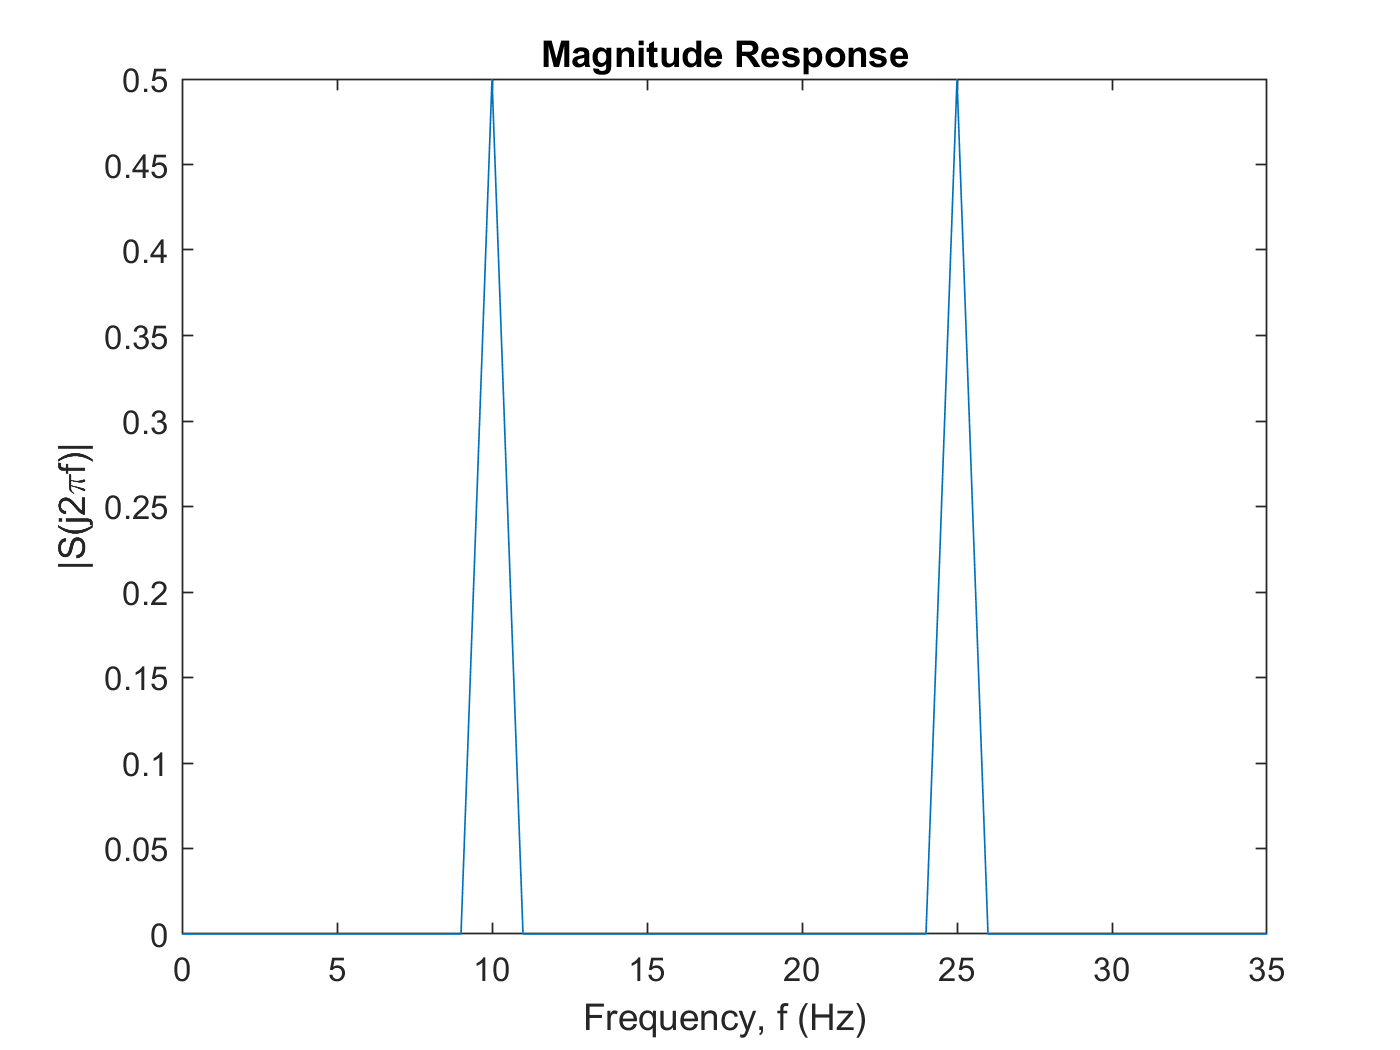
\includegraphics[width=\columnwidth]{SampleMagResponse.png}
    \caption{Right-half-plane plot of $\abs{\mathscr{F}\{s\}}$}   
    \label{SampleMagResponse}
\end{figure}

A time plot of and magnitude frequency spectrum for our modulated signal are given by Fig. \ref{ModTime} and Fig. \ref{ModMagResponse}, respectively.

\begin{figure}[ht]
	\centering
  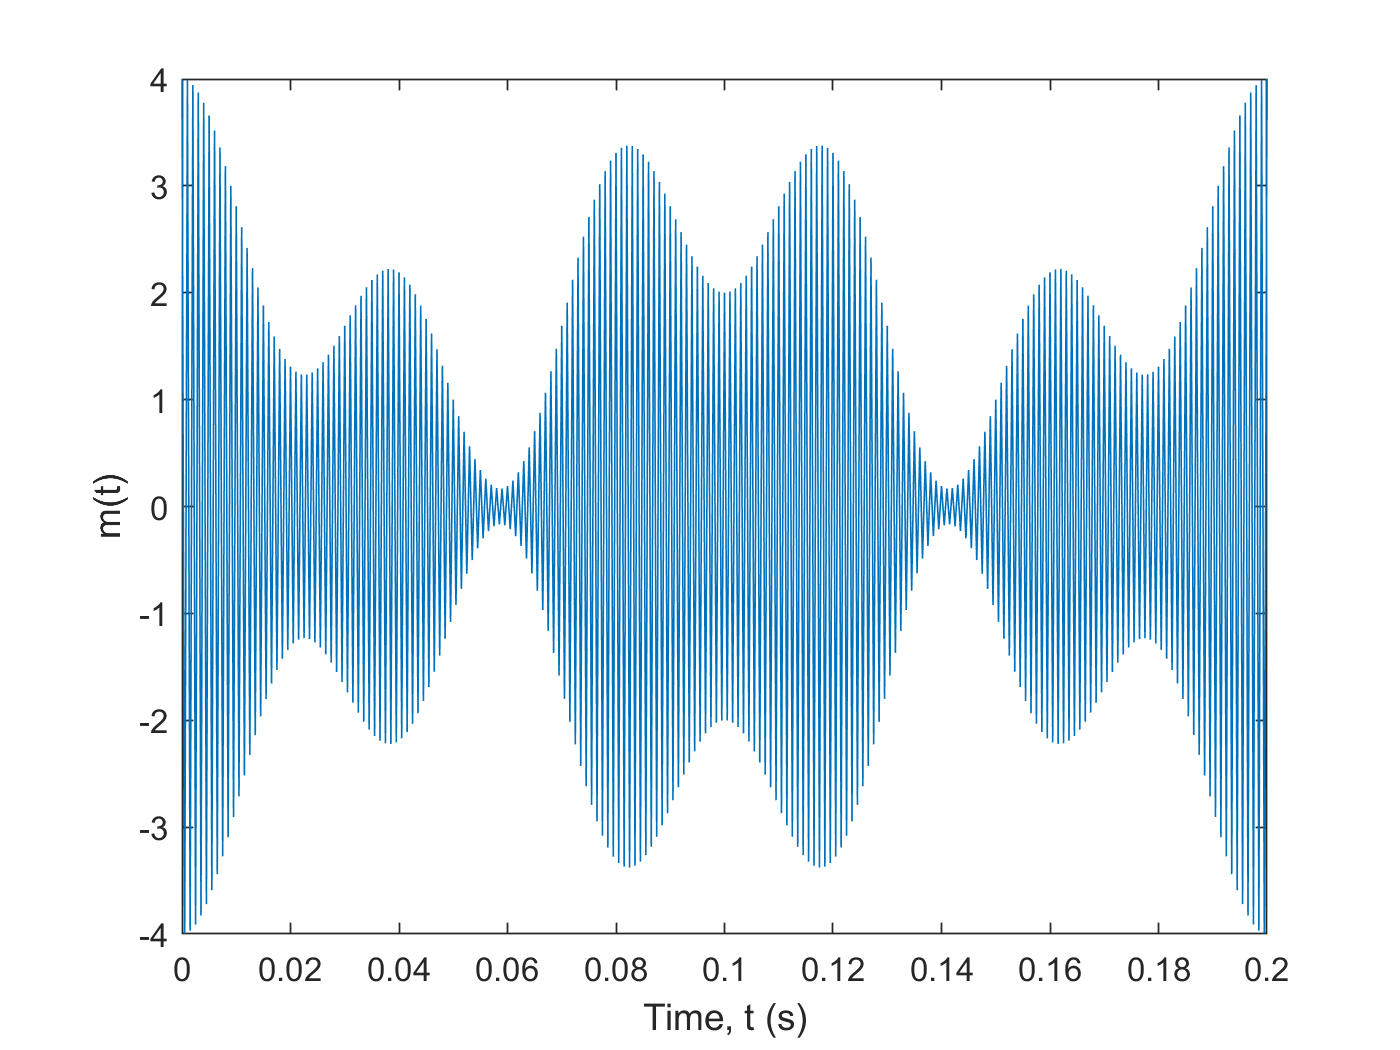
\includegraphics[width=\columnwidth]{MagTime.png}
    \caption{Our modulated signal, $m(t)$}
    \label{ModTime}
\end{figure}
    
\begin{figure}[h!]
	\centering
  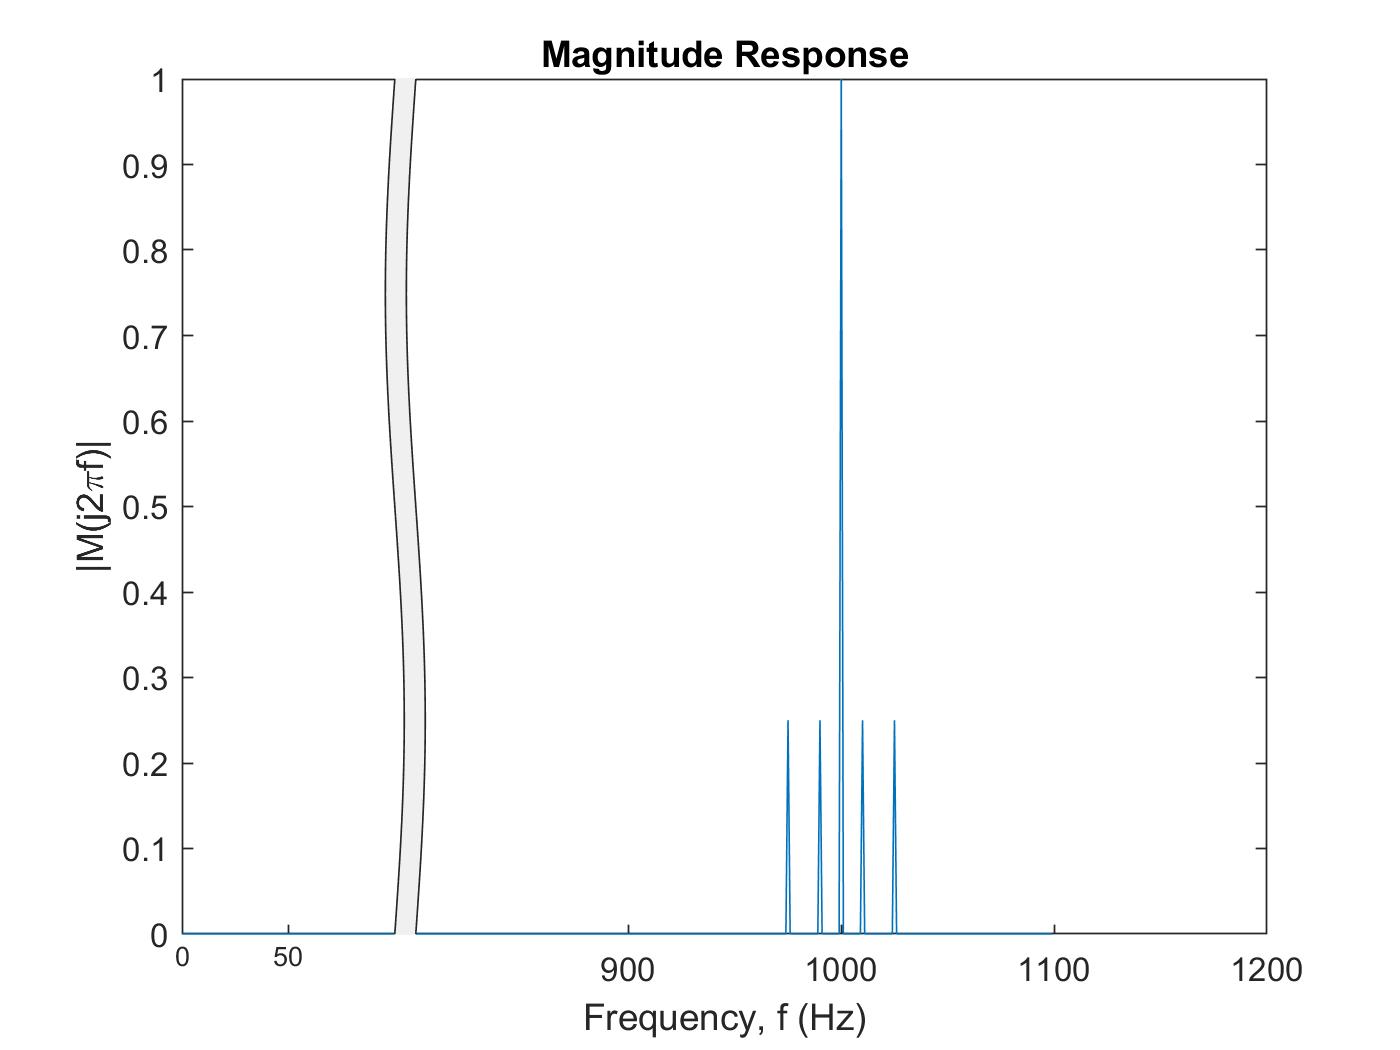
\includegraphics[width=\columnwidth]{MagResponse.png}
    \caption{Right-half-plane plot of $\abs{\mathscr{F}\{m\}}$}
    \label{ModMagResponse}
\end{figure}

\subsubsection{Retrieving the Modulated Signal}
To start, we need to isolate the modulated signal from the surrounding noise. We shall assume that a bandwidth of 2000Hz about our carrier signal is sufficient and that we do not need to worry about others broadcasting about our carrier frequency. We can accomplish this isolation by cutting off frequencies \SI{2000}{\hertz} about our carrier frequency via a bandpass filter formed by cascaded low- and high-pass filters. The transfer function resulting from cascading a first-order lowpass filter and a first-order highpass filter is given by eq. \eqref{BandpassCascade}.

\begin{equ}[ht]
    \begin{equation}    
    \begin{split}
        H\left(s\right)	&=H_{high}\left(s\right)H_{low}\left(s\right)\\
        				&=\frac{s}{s+\omega_{c_1}}\frac{\omega_{c_2}}{s+\omega_{c_2}}\\
                        &=\frac{s\omega_{c_2}}{s^2+s\left({\omega_c}_1+{\omega_c}_2\right)+\omega_{c_1}\omega_{c_2}}
        \end{split}
    \end{equation}
    \caption{Cascaded first-order highpass and lowpass filters}
    \label{BandpassCascade}
\end{equ}

However, we want to define things in terms of our carrier frequency (which for our purposes is the center frequency $\omega_0$) and bandwidth $\beta$. By the definitions of $\beta$ and $\omega_0$ given by eq. \eqref{BandwidthDef}, if we let $\omega_{c_2}\gg\omega_{c_1}$ we see that eq. \eqref{BandpassCascade} yields the transfer function noted in eq. \eqref{centerfreqdef}

\begin{align}
\beta &\coloneqq \omega_{c_2}-\omega_{c_1}\label{BandwidthDef}\\
\omega_0 &\coloneqq \sqrt{\omega_{c_2}\omega_{c_1}} \label{centerfreqdef}
\end{align}

\begin{equation}
    \begin{split}
	H(s)&=\frac{s\beta}{s^2+s\beta+\omega_{c_1}\omega_{c_2}}\\
    	&=\frac{s\beta}{s^2+s\beta+\omega_0^2}
    \end{split}
    \label{bandpasseq}
\end{equation}

If we require a filter of a higher order, we may cascade this filter with itself; i.e., we can obtain a bandpass filter of order $n$ by taking a bandpass filter of order $1$ and cascading it with itself $n$ times. While this results in increased rolloff (and thus $<\frac{1}{\sqrt{2}}$ at the corner frequencies) that depending on implementation may need to be considered, for our purposes the corner frequencies are sufficiently far enough away from the frequencies of our samples that we may ignore this.  As a result, for our purposes from eq. \eqref{bandpasseq} the transfer function for an $n$th-order bandpass filter can be as in eq. \eqref{nthBandpass}

\begin{equ}[ht]
    \begin{equation}    
    H_{n}(s)=H_{1}(s)^n=\left(\frac{s\beta}{s^2+s\beta+\omega_0^2}\right)^n
    \label{nthBandpass}
    \end{equation}
    \caption{nth-order bandpass filter with unspecified rolloff}
\end{equ}


\subsubsection{Half-wave Rectification}
As seen in Fig. \ref{ModMagResponse} and discussed in the modulation section, an extracted modulated signal has the original sample signal's constituent frequencies shifted by the carrier wave's frequency so that in the response plot their corresponding peaks are centered about it as if it were the origin. Consequently, we use half-wave rectification to bring those frequencies back about $\SI{0}{Hz}$. Given the signal, carrier, and modulation as defined in part B.2 (eqs. \eqref{sample}, \eqref{carrier}, \eqref{modulated}), applying half-wave rectification we retrieve a signal with time and magnitude response plots given by Figs. \ref{RectifiedTime}, \ref{RectifiedResponse}.

\begin{figure}[ht]
	\centering
 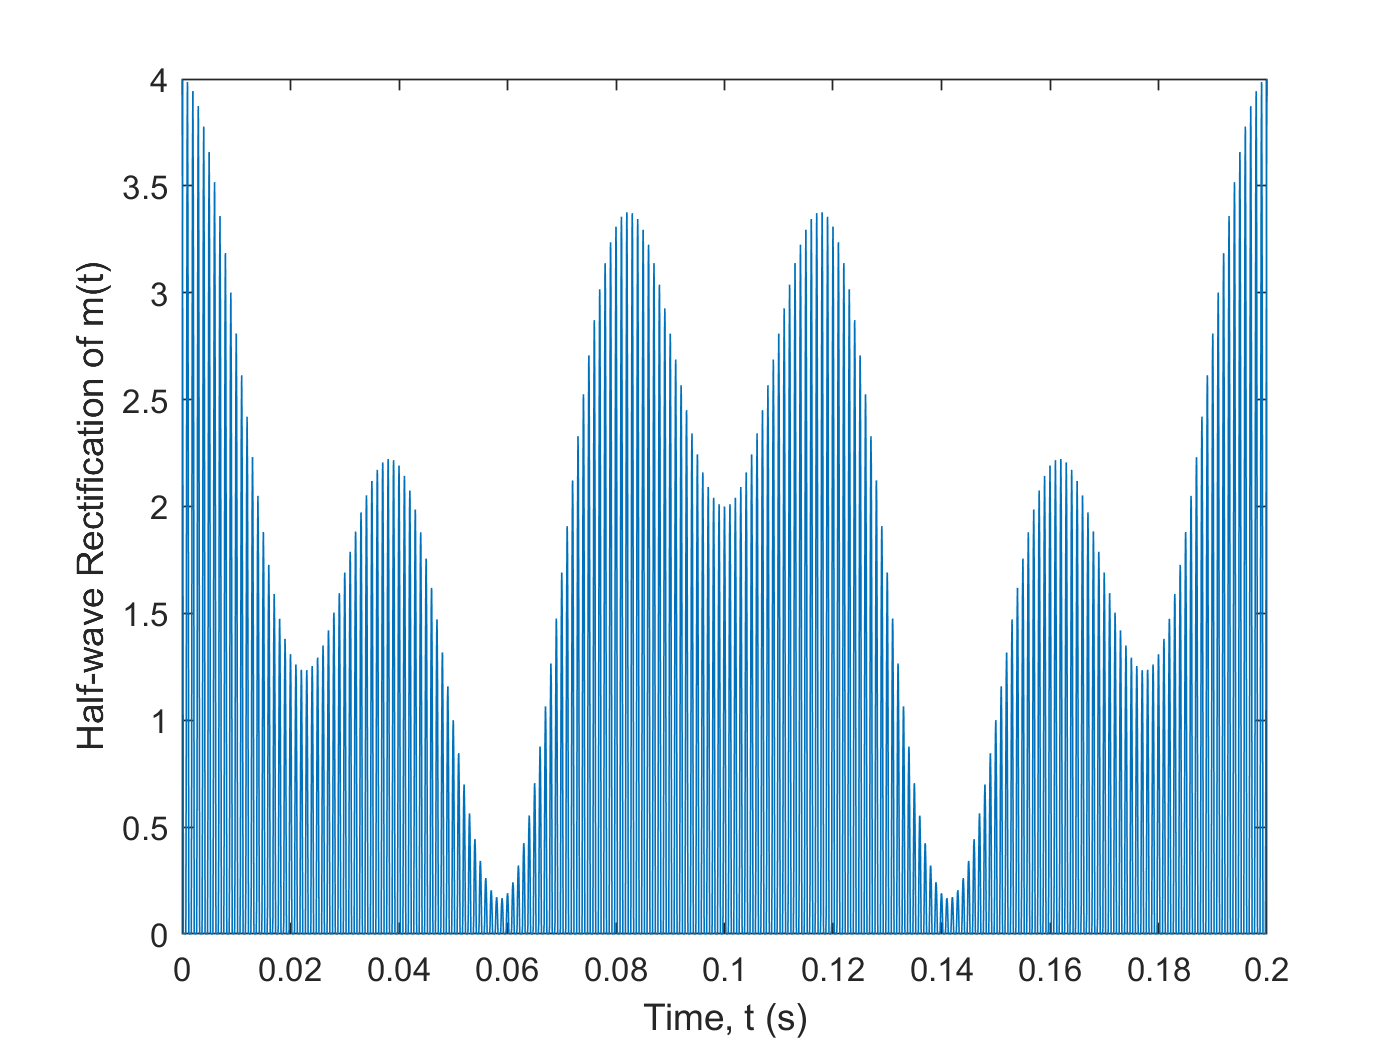
\includegraphics[width=\columnwidth]{HalfWaveTime.png}
    \caption{Rectified retrieved signal}
    \label{RectifiedTime}
\end{figure}

\begin{figure}[ht]
	\centering
  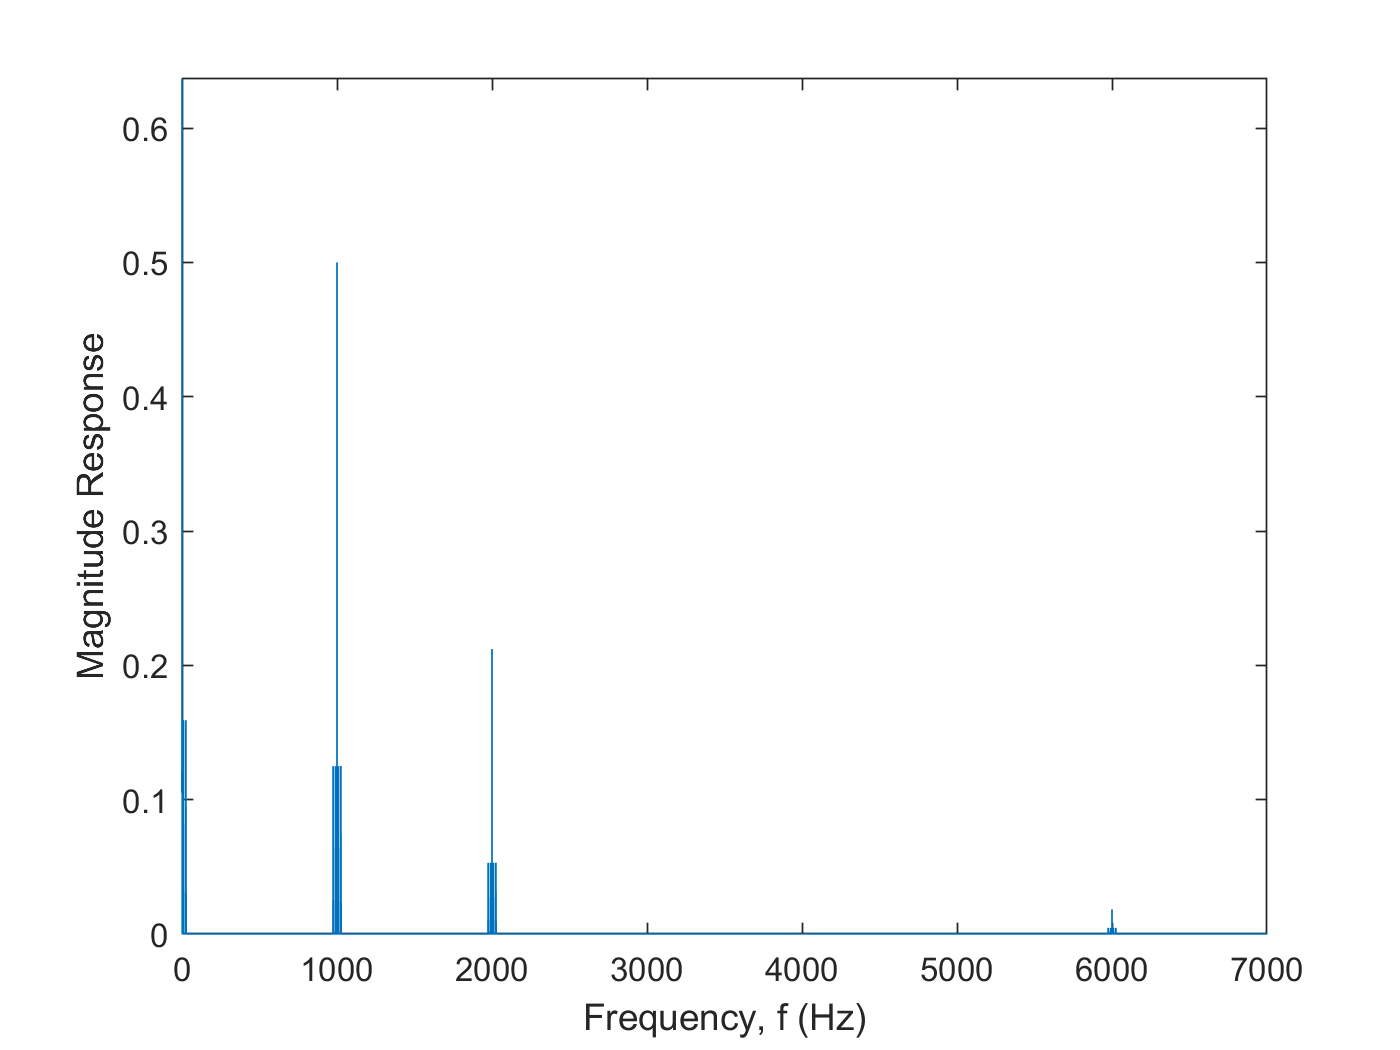
\includegraphics[width=\columnwidth]{HalfWaveMag.png}
    \caption{Magnitude response of the rectified retrieved signal}   
    \label{RectifiedResponse}
\end{figure}


\subsubsection{Low-pass Filtering}
As seen in Figs. \ref{RectifiedTime} and \ref{RectifiedResponse}, half-wave rectifying a modulated wave leaves jagged holes within the wave in the time domain corresponding to residual peaks away from the origin in the frequency domain. To remedy this, we low-pass the desired frequencies below some threshold, eliminating the other peaks. Given our ongoing example, we choose a low-pass filter with a cutoff frequency of \SI{500}{\hertz} to obtain (through the process outlined in Appendix A) the transfer function given in eq. \eqref{500HzLowPass} and whose magnitude and frequency response plots are given by Fig. \ref{500HzLPFBode}.
\begin{equation}
    \resizebox{\columnwidth}{!}{%
$H(s)=\frac{9.74091\times 10^{13}}{s^4+8209.38 s^3+3.36969\times 10^7 s^2+8.10233\times 10^{10} s+9.74091\times 10^{13}}$%
}
\label{500HzLowPass}
\end{equation}

\begin{figure}[ht]
	\centering
 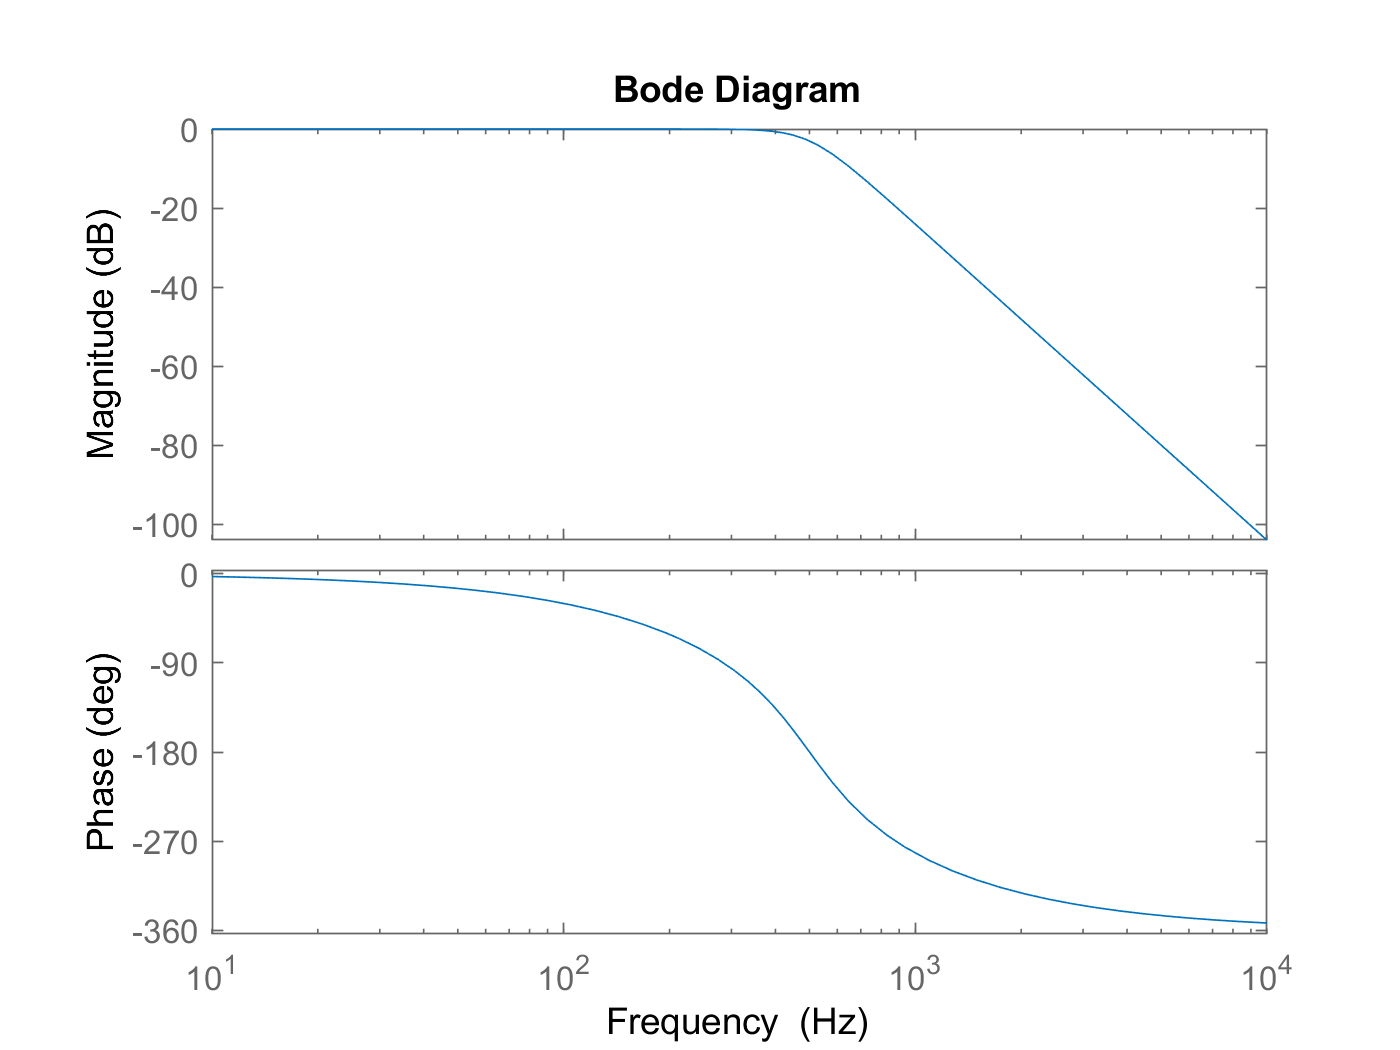
\includegraphics[width=\columnwidth]{500HzLPFBode.png}
    \caption{Bode plot of the 500Hz second-order low-pass Butterworth filter given by eq. \eqref{500HzLowPass}}
    \label{500HzLPFBode}
\end{figure}

Applying this filter to our example, we obtain the time and magnitude response plots given by Figs. \ref{lowpasstime}, \ref{lowpassmagresponse}.
\begin{figure}[ht]
	\centering
 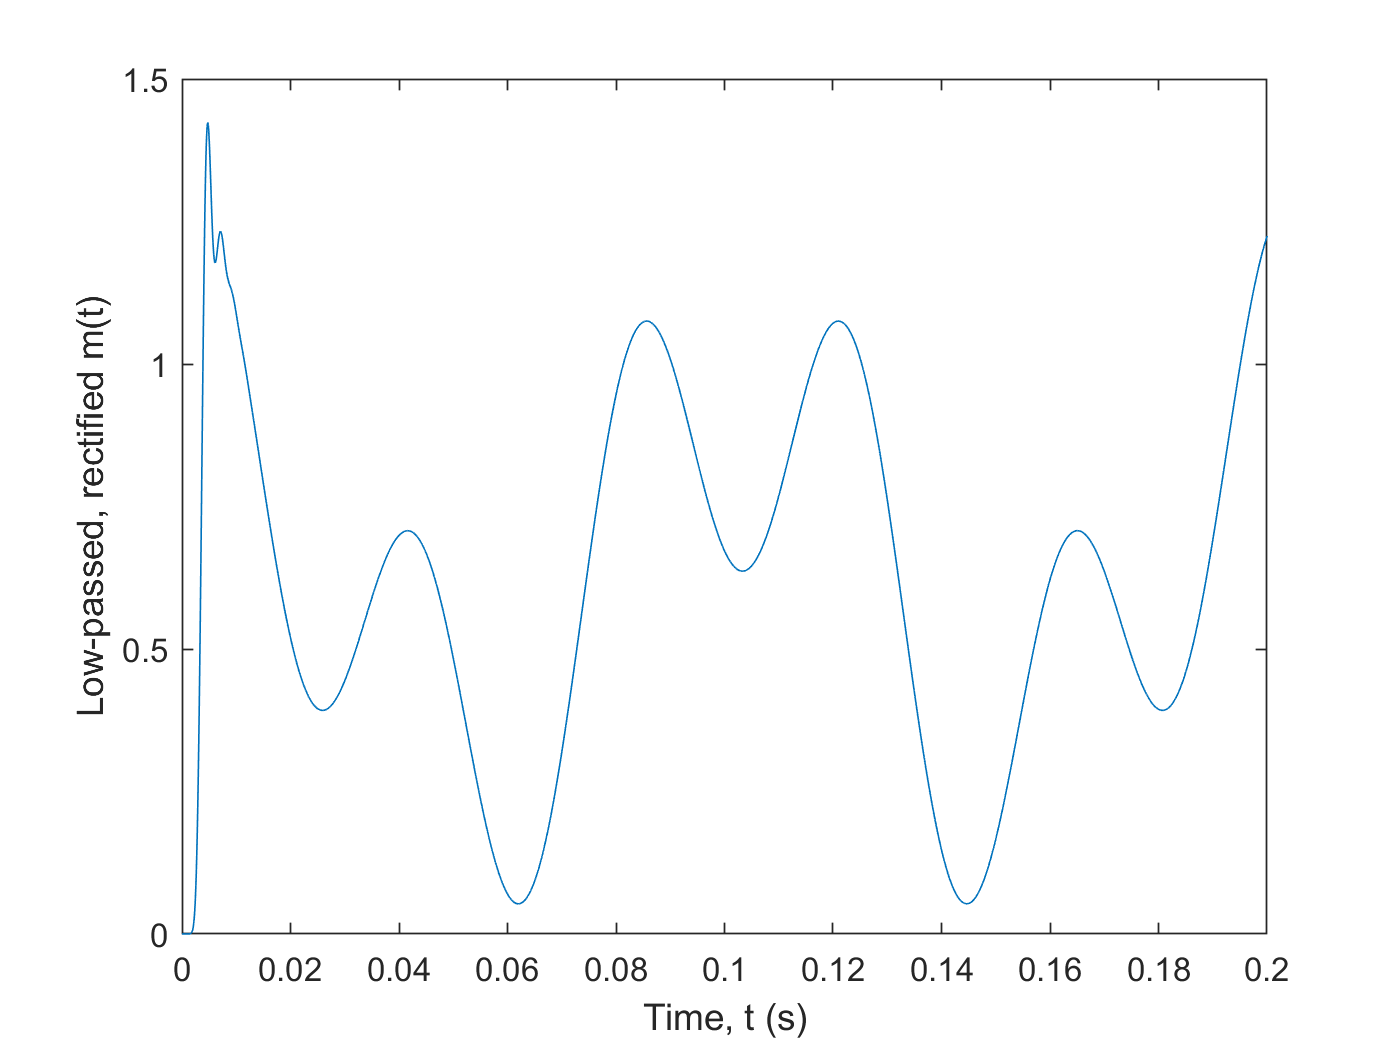
\includegraphics[width=\columnwidth]{LowPassTime.png}
    \caption{Low-passed, rectified, retrieved signal}
    \label{lowpasstime}
\end{figure}

\begin{figure}[ht]
	\centering
  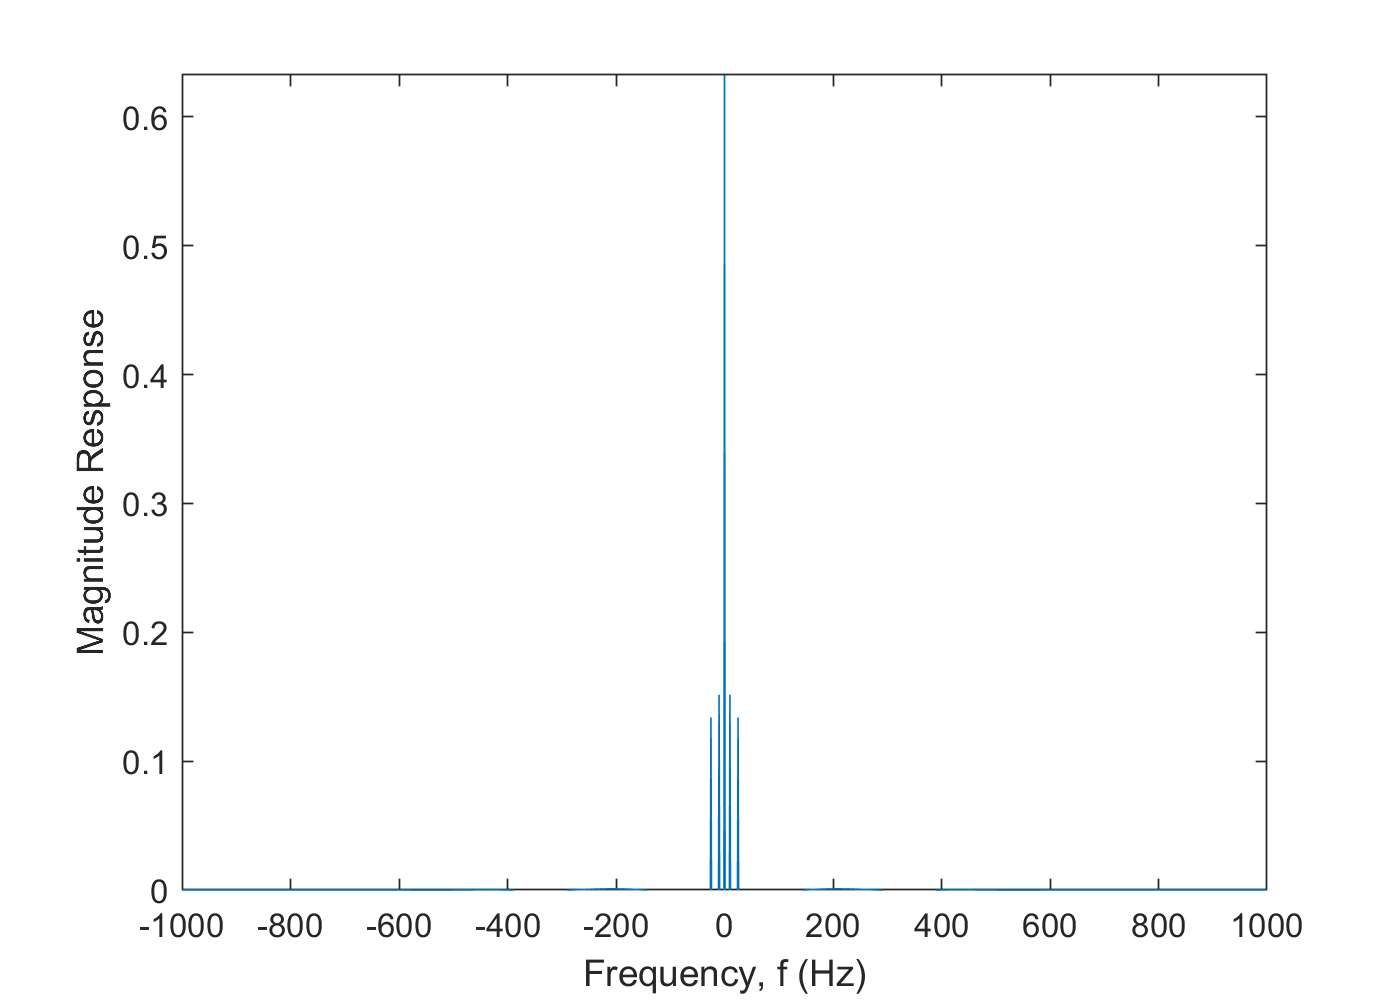
\includegraphics[width=\columnwidth]{LowPassMag.png}
    \caption{Magnitude response of the low-passed, rectified, retrieved signal}   
    \label{lowpassmagresponse}
\end{figure}

\subsubsection{Mean Removal}
Finally, looking at Figs. \ref{lowpasstime}, \ref{lowpassmagresponse}, we see that we need to remove our original DC offset to retrieve our original sample. We can remove the center magnitude response spike/time domain magnitude offset that brings it above the time-axis caused by our DC offset by removing the mean from the low-passed signal. Doing so, we see in Figs. \ref{meanremovetime}, \ref{meanremovemagresponse} that other than a small initial spike in the time domain, we have (approximately) retrieved our original sample signal.

\begin{figure}[ht]
	\centering
 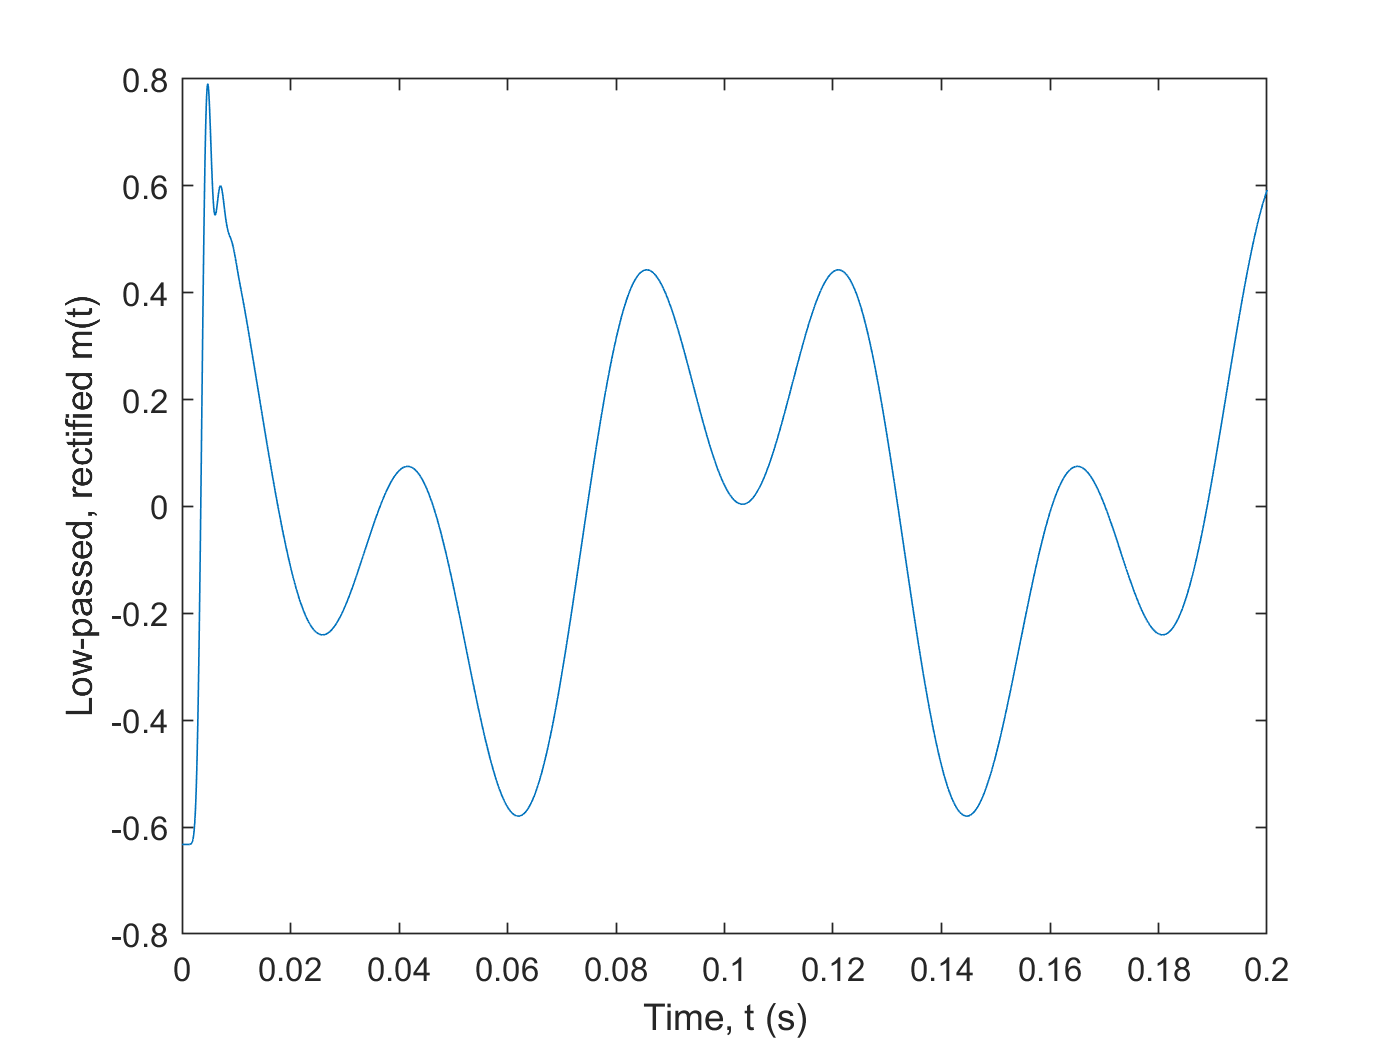
\includegraphics[width=\columnwidth]{meanremovedtime.png}
    \caption{Mean-removed, low-passed, rectified, retrieved signal}
    \label{meanremovetime}
\end{figure}

\begin{figure}[ht]
	\centering
  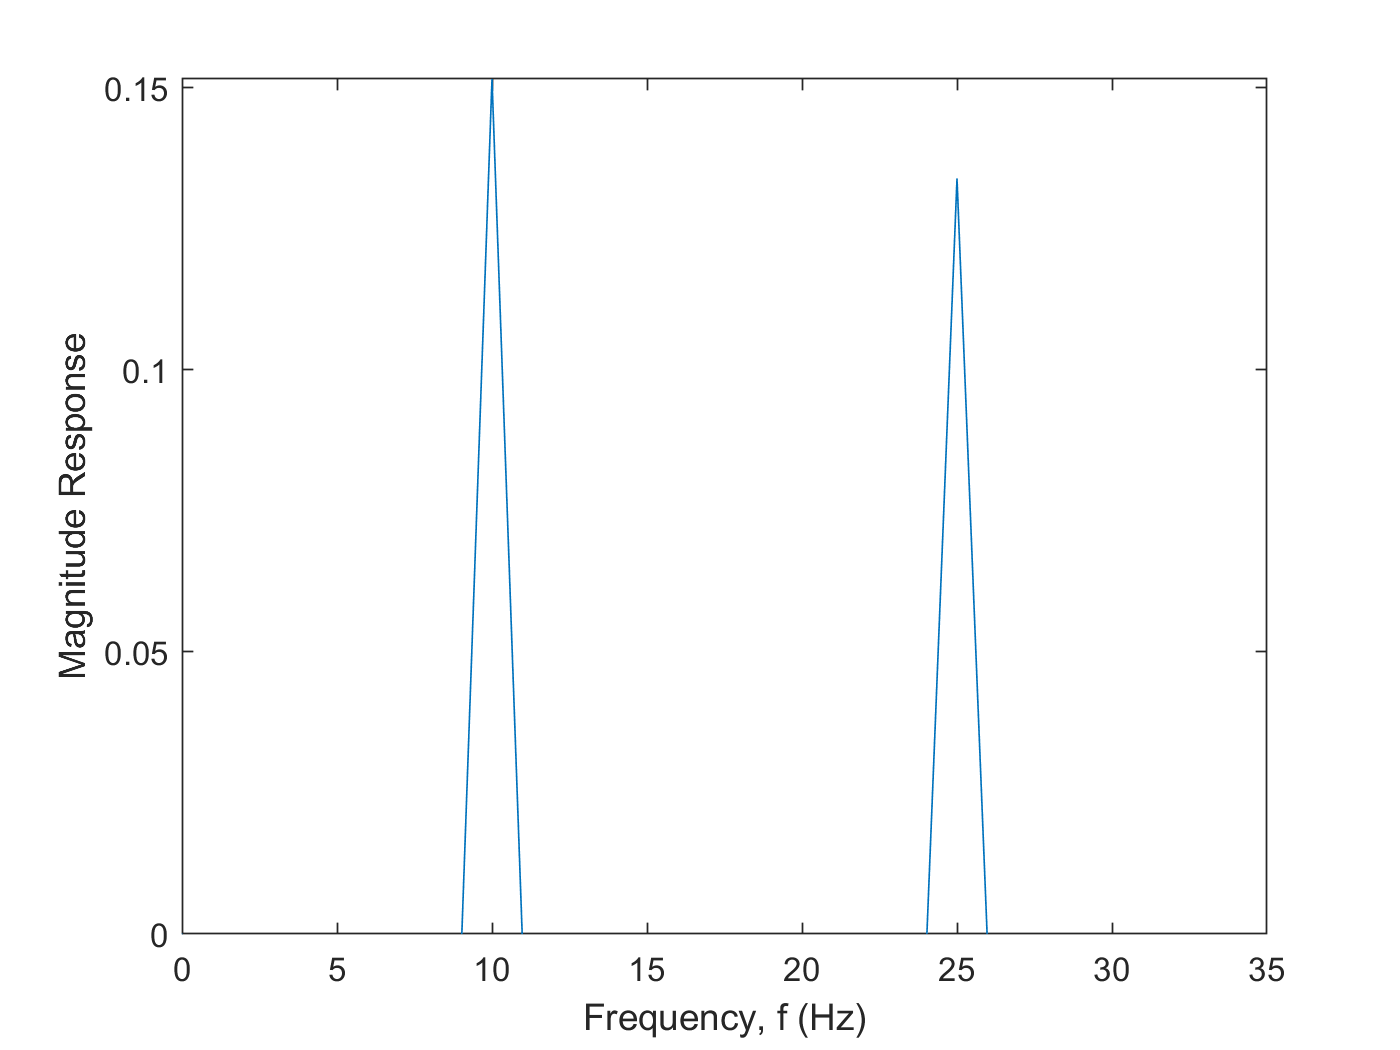
\includegraphics[width=\columnwidth]{meanremovedmag.png}
    \caption{Magnitude response of the mean-removed, low-passed, rectified, retrieved signal}   
    \label{meanremovemagresponse}
\end{figure}

\subsubsection{Applying this to our audio samples}
We repeat the process outlined in the above subsubsections with a provided collection of modulated signals of recordings of a professor speaking the letters of the NATO Phonetic Alphabet, each recorded at a sample rate 8000Hz with allocated bandwidth 2000Hz and on carrier frequencies ranging from 20kHz through 132.5kHz at 4.5kHz intervals. As explained in the subsection Retrieving the Modulated Signal, we use eq. \eqref{nthBandpass} to obtain a bandpass filter with the transfer function given by eq. \eqref{finaltransferfunc} and whose magnitude and frequency response plots are given by Figs. \ref{bpfBode}, \ref{bpfBodeZoomed}. We then perform half-wave rectification in accordance with the description given in the subsection with the same name, Half-wave Rectification. Next, as described by the subsection Low-pass Filtering, we design a 4th-order Butterworth low-pass filter with cutoff frequency \SI{2000}{\hertz} given by eq. \eqref{2000HzLowPass} and whose magnitude and frequency response are given by Figs. \ref{lpfBode}, \ref{lpfBodeZoomed} using the process given in Appendix A, and later apply mean removal as clarified in the subsection Mean Removal. We require one extra step, as the signal we have been provided has been upsampled from 8000Hz to 320000 Hz, so we decimate (downsample) the symbol back down to 8000Hz. Finally, we record at which frequency each spoken NATO Phonetic Alphabet letter was modulated over.

\begin{equation}
H\left(s\right)=\left(\frac{2000\cdot2\pi s}{s^2+2000\cdot2\pi s+\omega_{carrier}^2}\right)^2
\label{finaltransferfunc}
\end{equation}

\begin{figure}[ht]
	\centering
 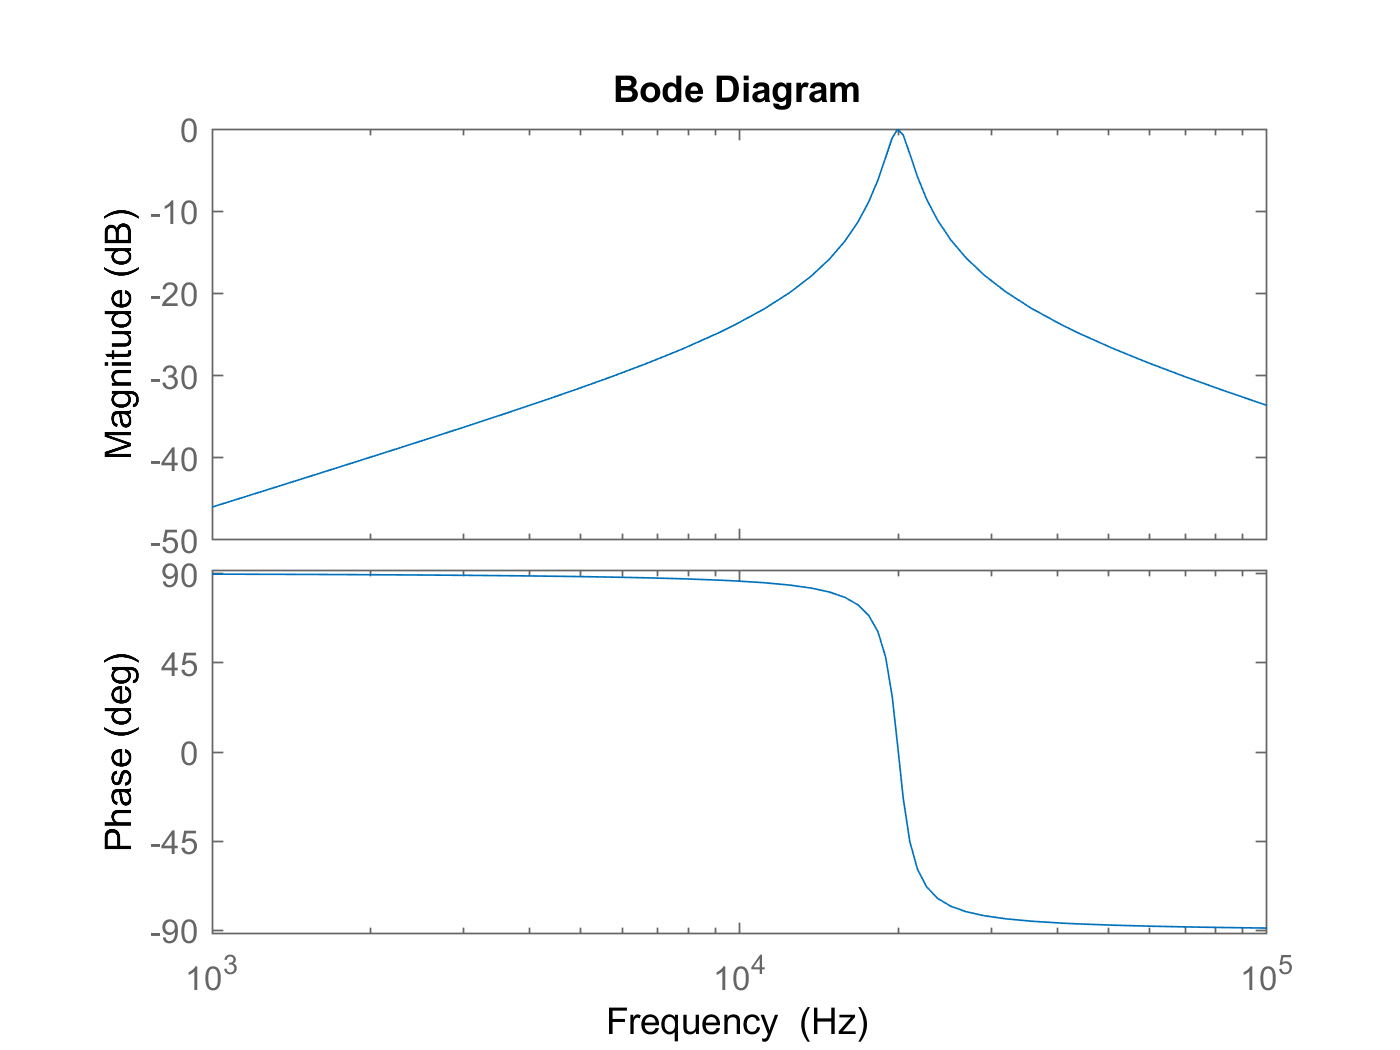
\includegraphics[width=\columnwidth]{bpfBode.png}
    \caption{Bode plot of the second-order Butterworth bandpass filter with center frequency \SI{20}{\kilo\hertz} and bandwidth \SI{2}{\kilo\hertz} given by eq. \eqref{finaltransferfunc}}
    \label{bpfBode}
\end{figure}

\begin{figure}[ht]
	\centering
  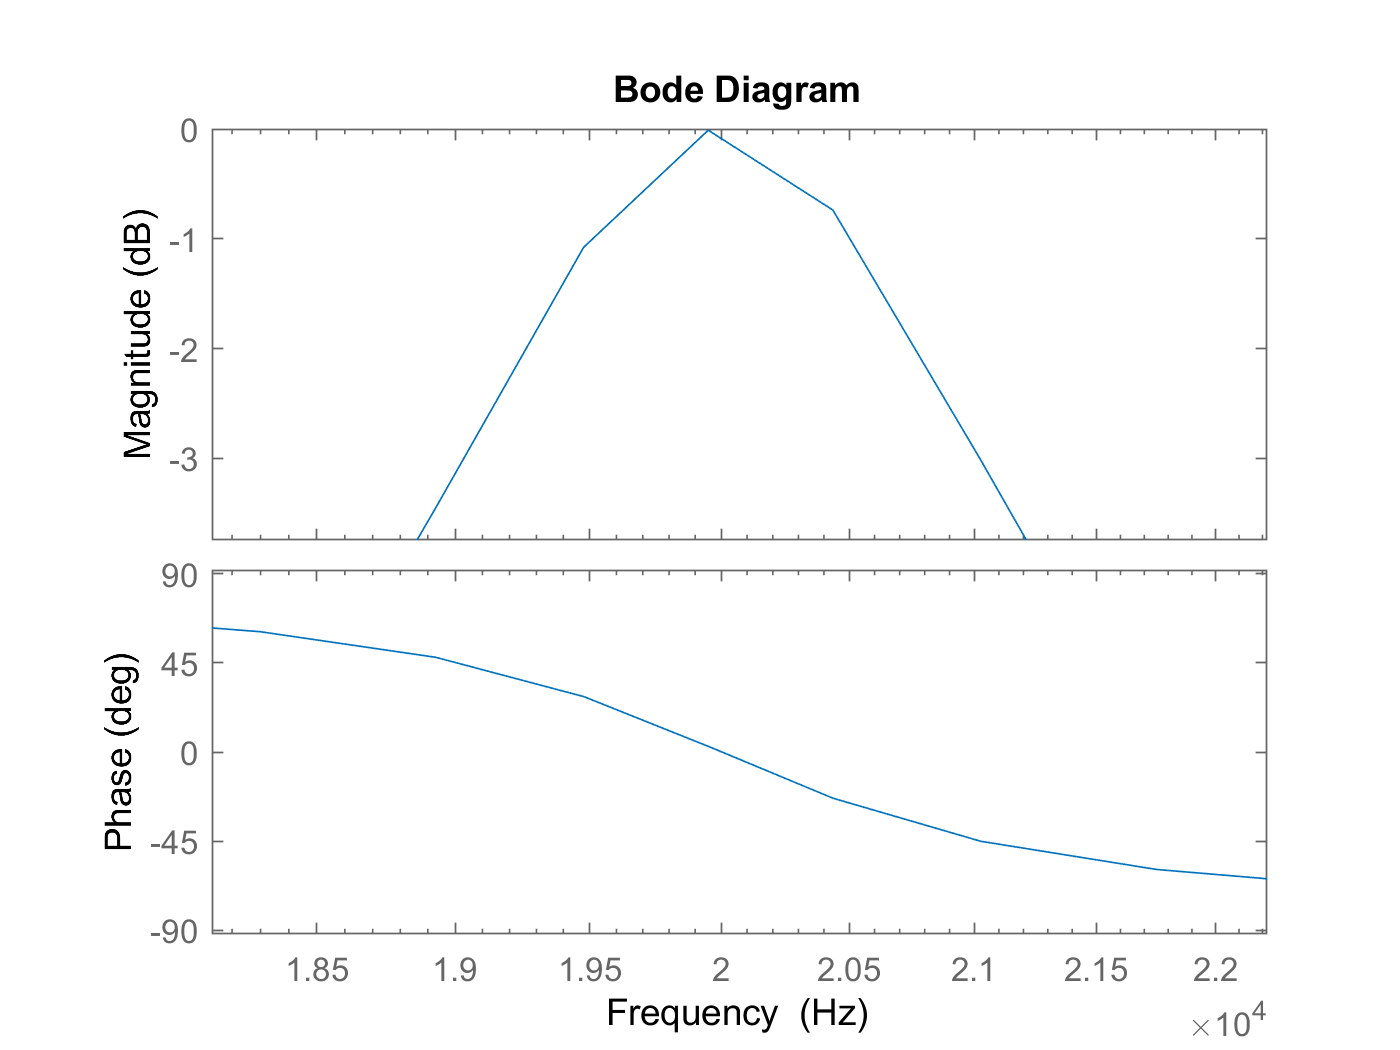
\includegraphics[width=\columnwidth]{bpfBodeZoomed.png}
    \caption{Bode plot of the second-order Butterworth bandpass filter with center frequency \SI{20}{\kilo\hertz} and bandwidth \SI{2}{\kilo\hertz} given by eq. \eqref{finaltransferfunc} (zoomed in to show -3dB cutoffs)}   
    \label{bpfBodeZoomed}
\end{figure}

\begin{equation}
    \resizebox{\columnwidth}{!}
    {$%
H(s)=\frac{2.49367\times 10^{16}}{s^4+32837.5 s^3+5.39151\times 10^8 s^2+5.18549\times 10^{12} s+2.49367\times 10^{16}}%
$}
\label{2000HzLowPass}
\end{equation}

\begin{figure}[ht]
	\centering
 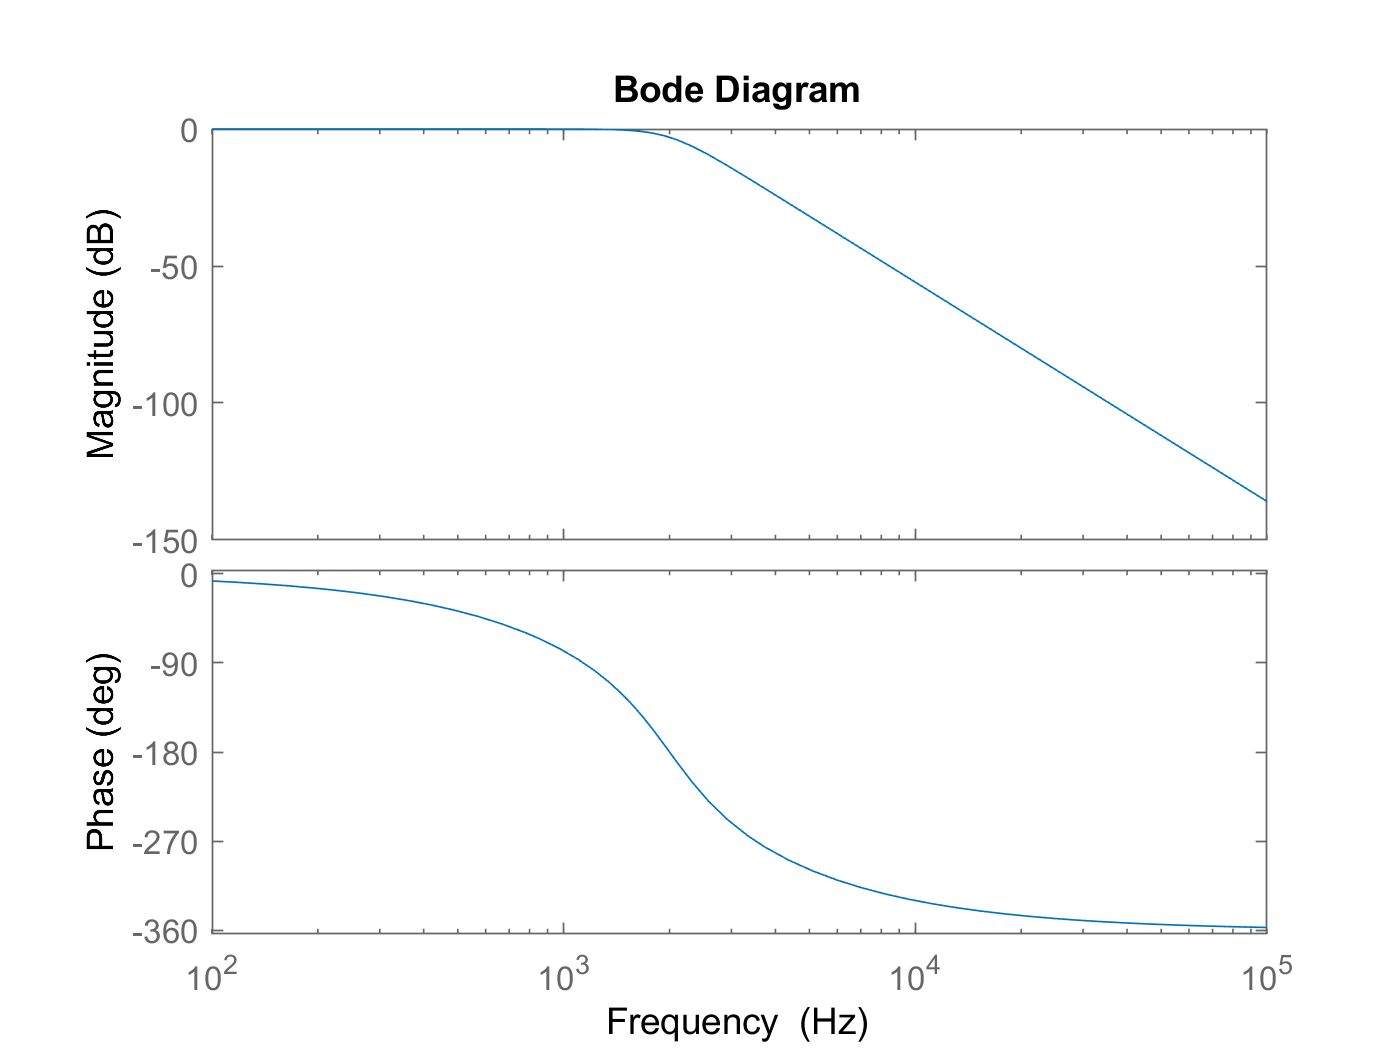
\includegraphics[width=\columnwidth]{lpfBode.png}
    \caption{Bode plot of the fourth-order Butterworth lowpass filter with cutoff frequency \SI{2}{\kilo\hertz} given by eq. \eqref{2000HzLowPass}}
    \label{lpfBode}
\end{figure}

\begin{figure}[ht]
	\centering
  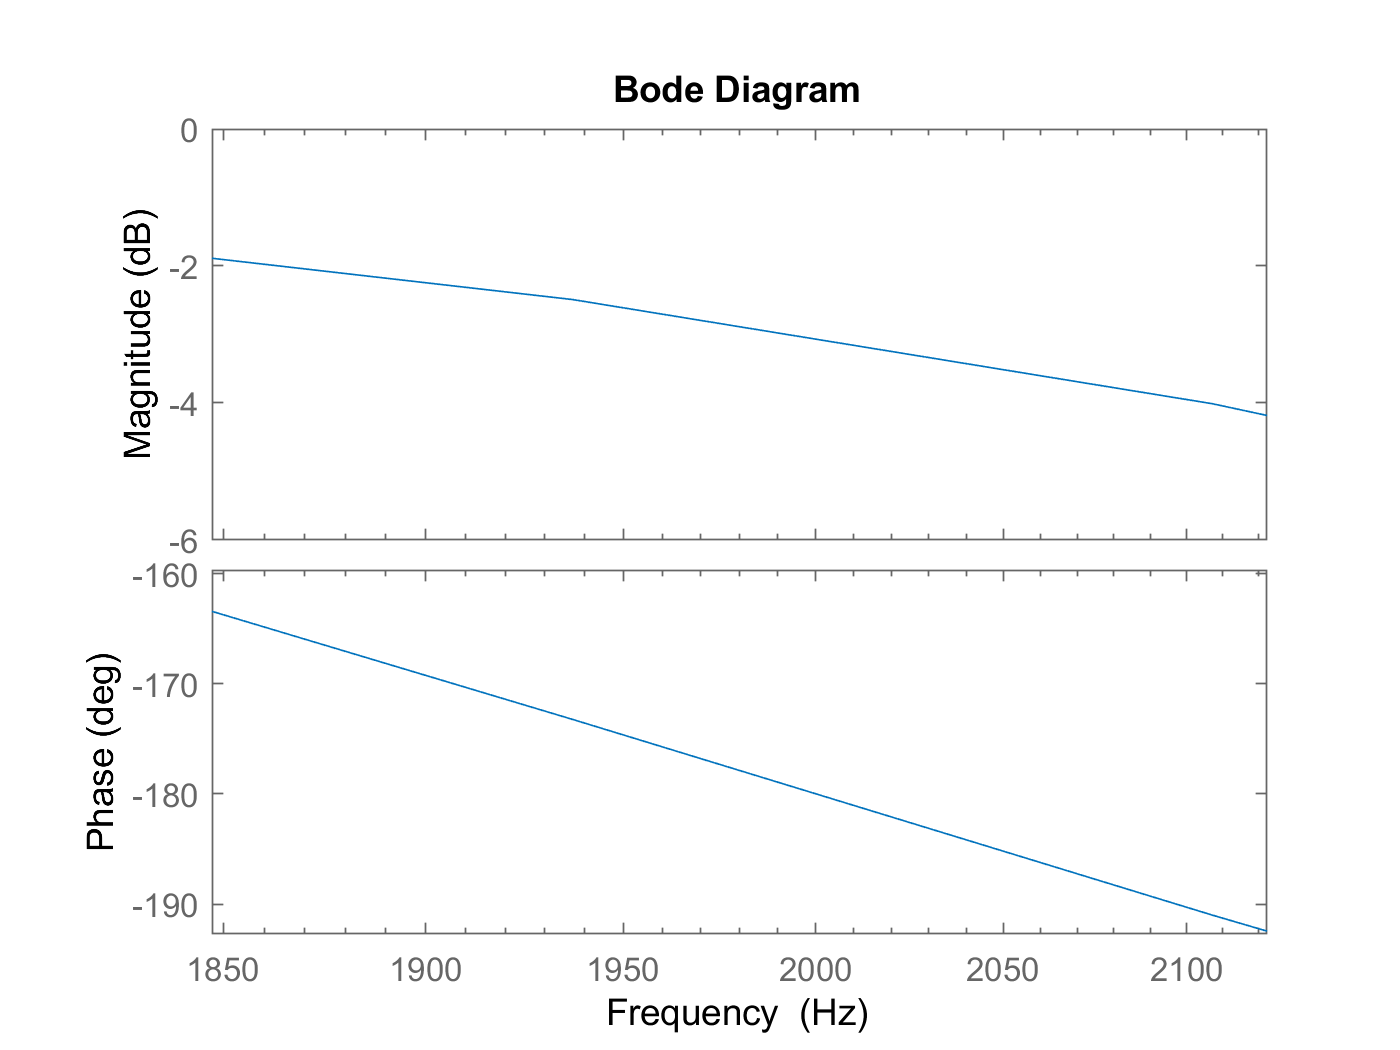
\includegraphics[width=\columnwidth]{lpfBodeZoomed.png}
    \caption{Bode plot of the fourth-order Butterworth lowpass filter with cutoff frequency \SI{2}{\kilo\hertz} given by eq. \eqref{2000HzLowPass} (zoomed in to show -3dB cutoff)}   
    \label{lpfBodeZoomed}
\end{figure}




\section{Results}
\subsection{Time and Magnitude Response Graphs for Demodulated Signal Carried by 20kHz Carrier}
The results of performing our demodulation process on the provided collection of modulated signals of recordings of a professor speaking the letters of the NATO Phonetic Alphabet (each recorded at a sample rate 8000Hz with allocated bandwidth 2000Hz and on carrier frequencies ranging from 20kHz through 132.5kHz at 4.5kHz intervals) is demonstrated by Figs. \ref{JulietBandpass}, \ref{JulietHalfWave}, \ref{JulietLowpassUnzoomed}, \ref{JulietLowpassZoomed}, \ref{JulietMeanRemoved}, \ref{JulietTime}. 
\begin{figure}[!htb]
	\centering
  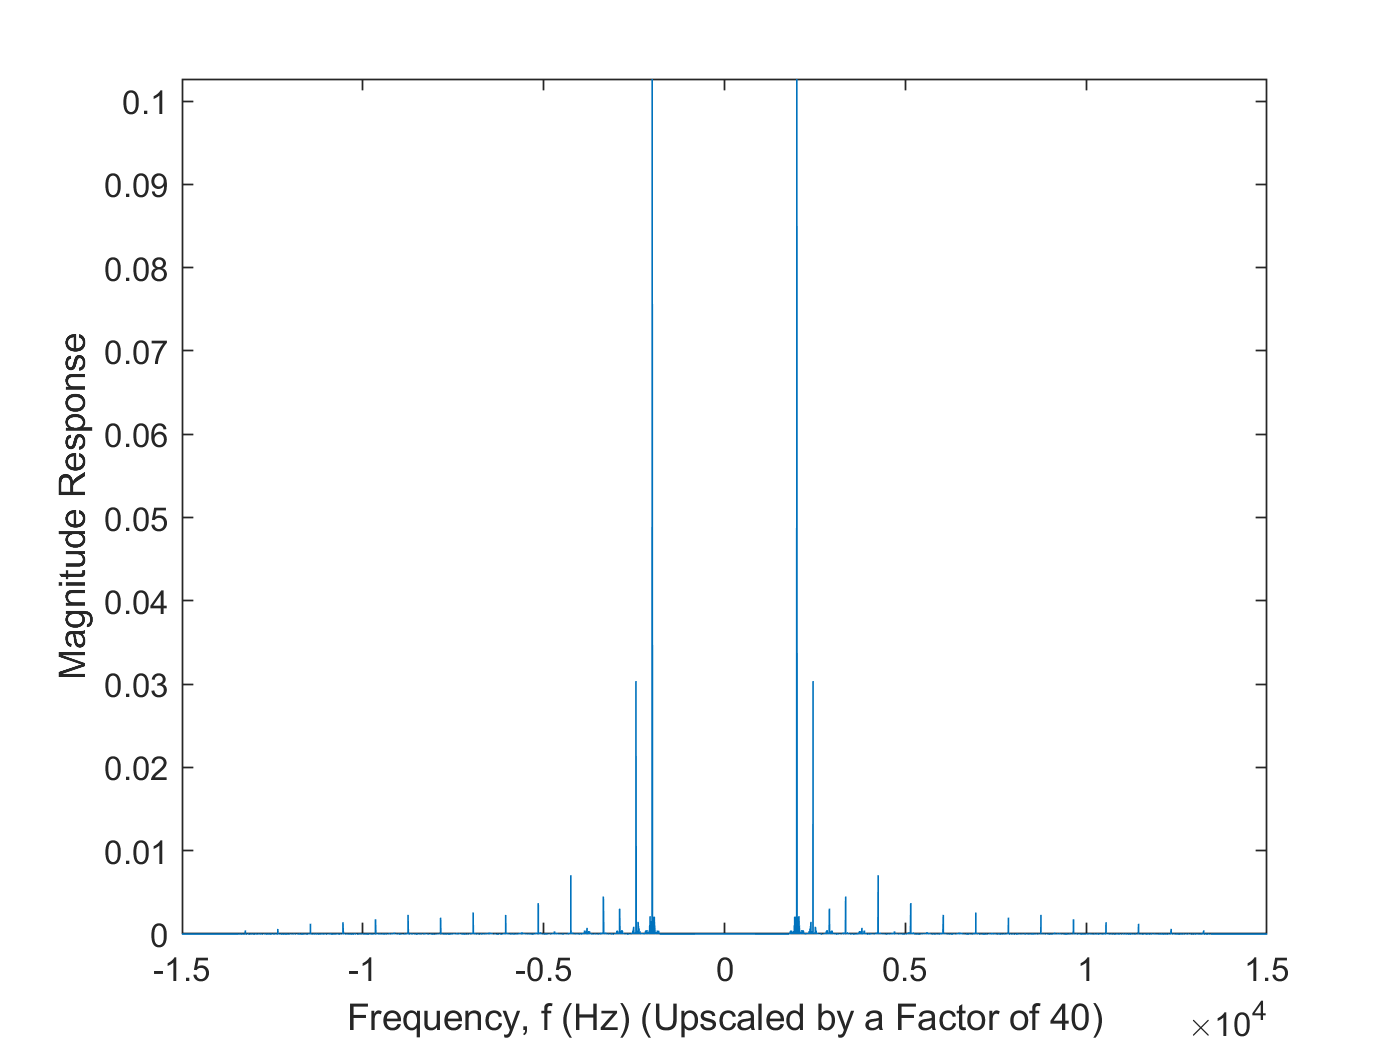
\includegraphics[width=\columnwidth]{JulietBandpassMag.png}
    \caption{Magnitude response for 20kHz-carried modulated signal (Juliet)}   
    \label{JulietBandpass}
\end{figure}

\begin{figure}[!htb]
	\centering
  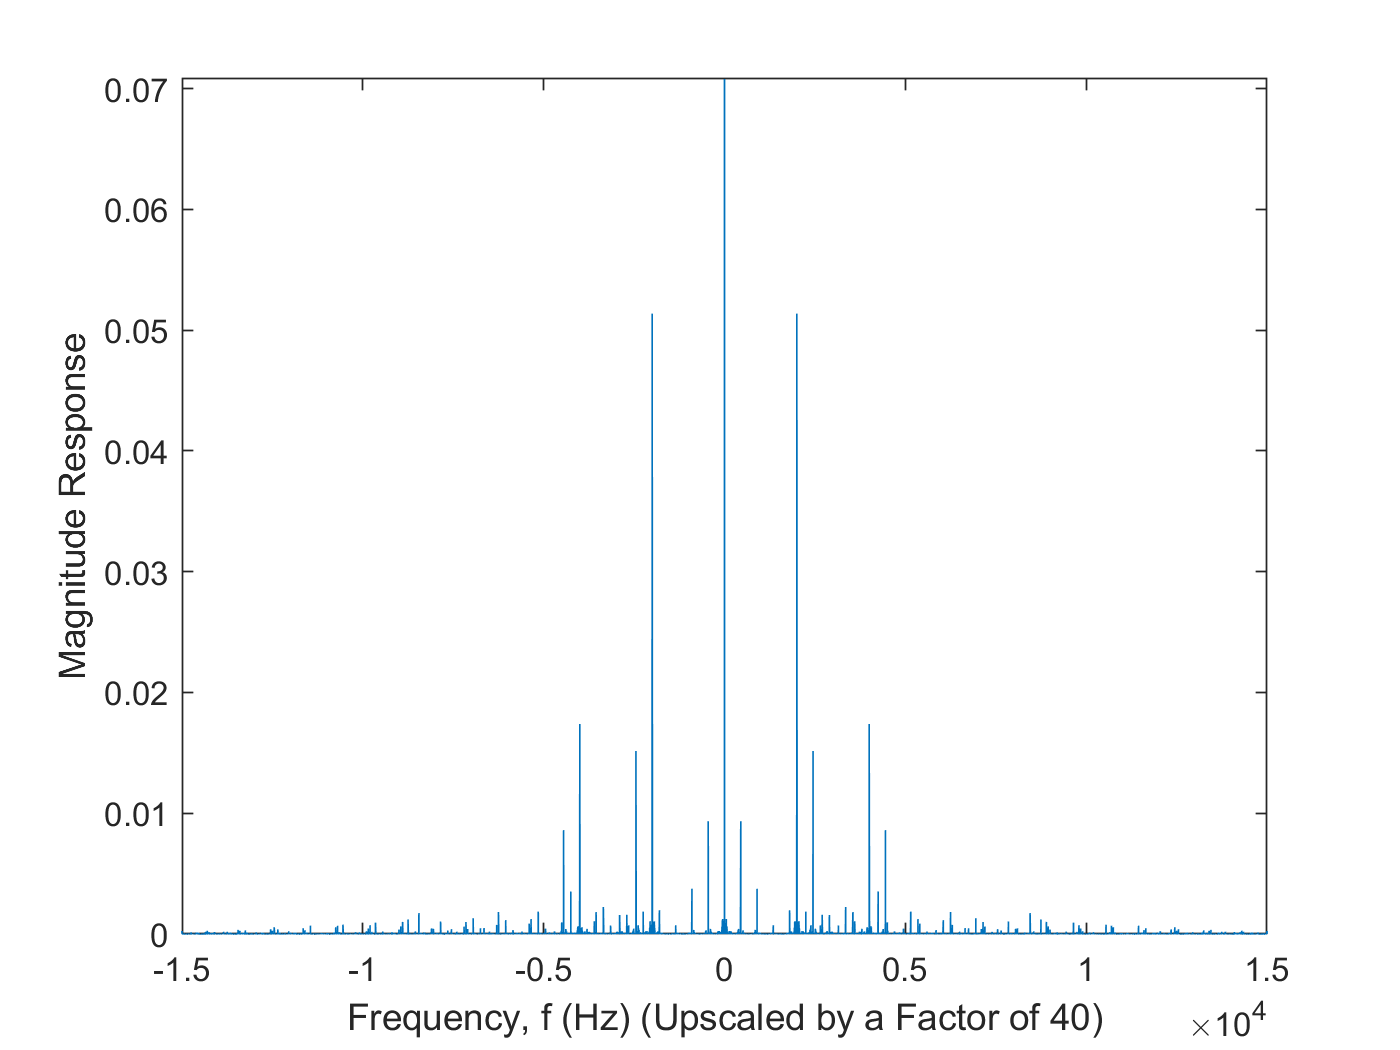
\includegraphics[width=\columnwidth]{JulietHalfWaveMag.png}
    \caption{Magnitude response for 20kHz-carried modulated signal (Juliet) after half-wave rectification step}   
    \label{JulietHalfWave}
\end{figure}

\begin{figure}[!htb]
	\centering
  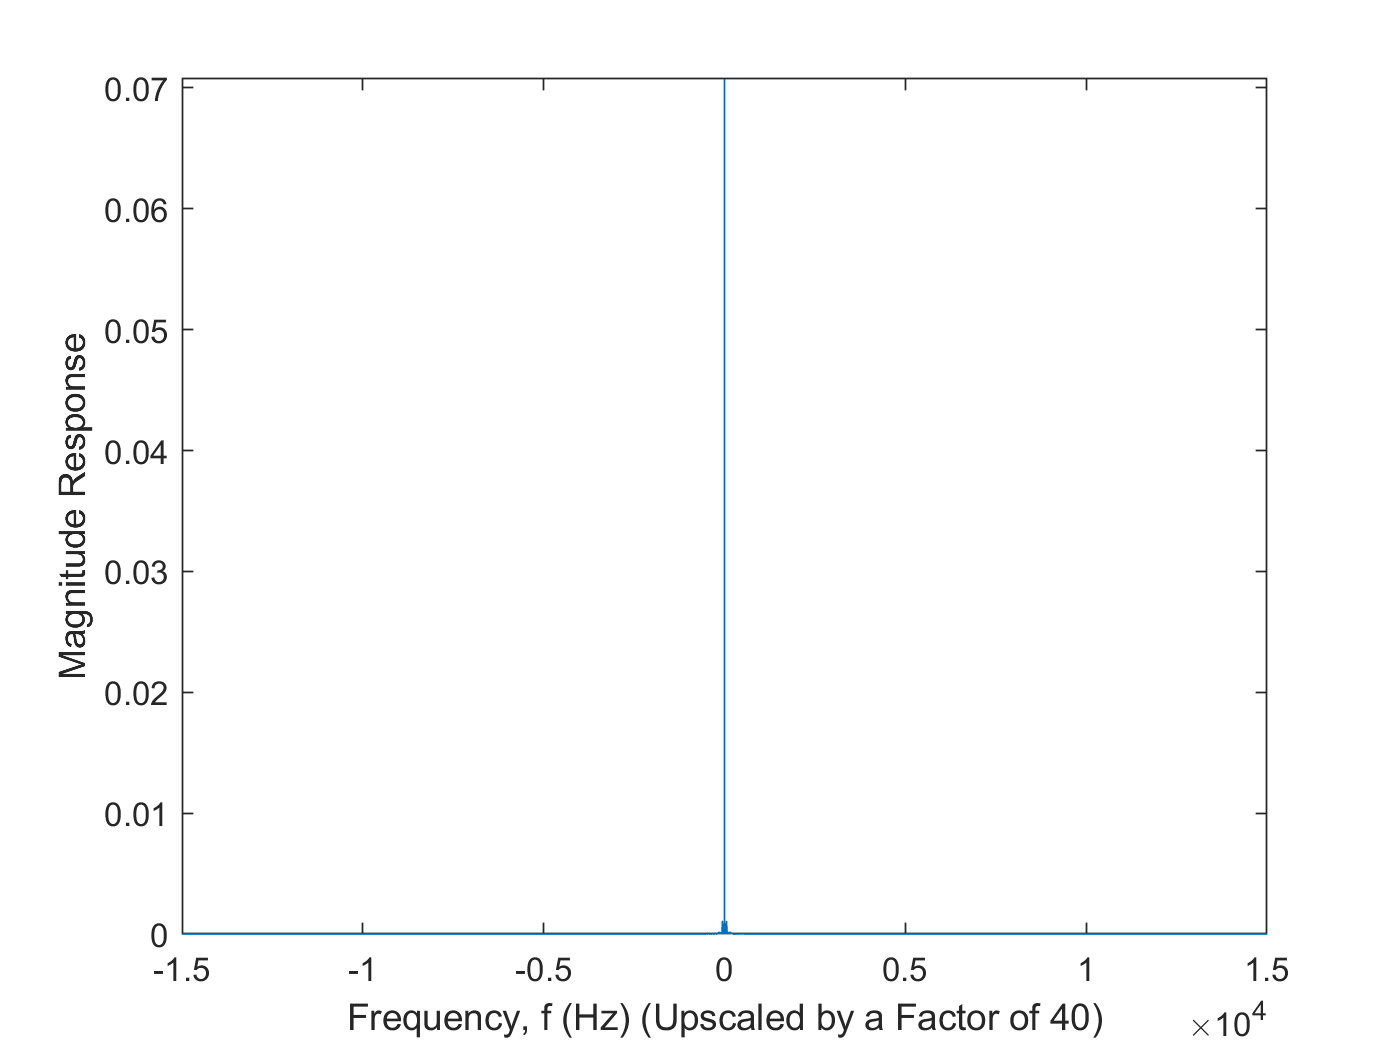
\includegraphics[width=\columnwidth]{JulietLowPassMagUnzoomed.png}
    \caption{Magnitude response for 20kHz-carried modulated signal (Juliet) after low-pass step (unzoomed)}   
    \label{JulietLowpassUnzoomed}
\end{figure}

\begin{figure}[!htb]
	\centering
  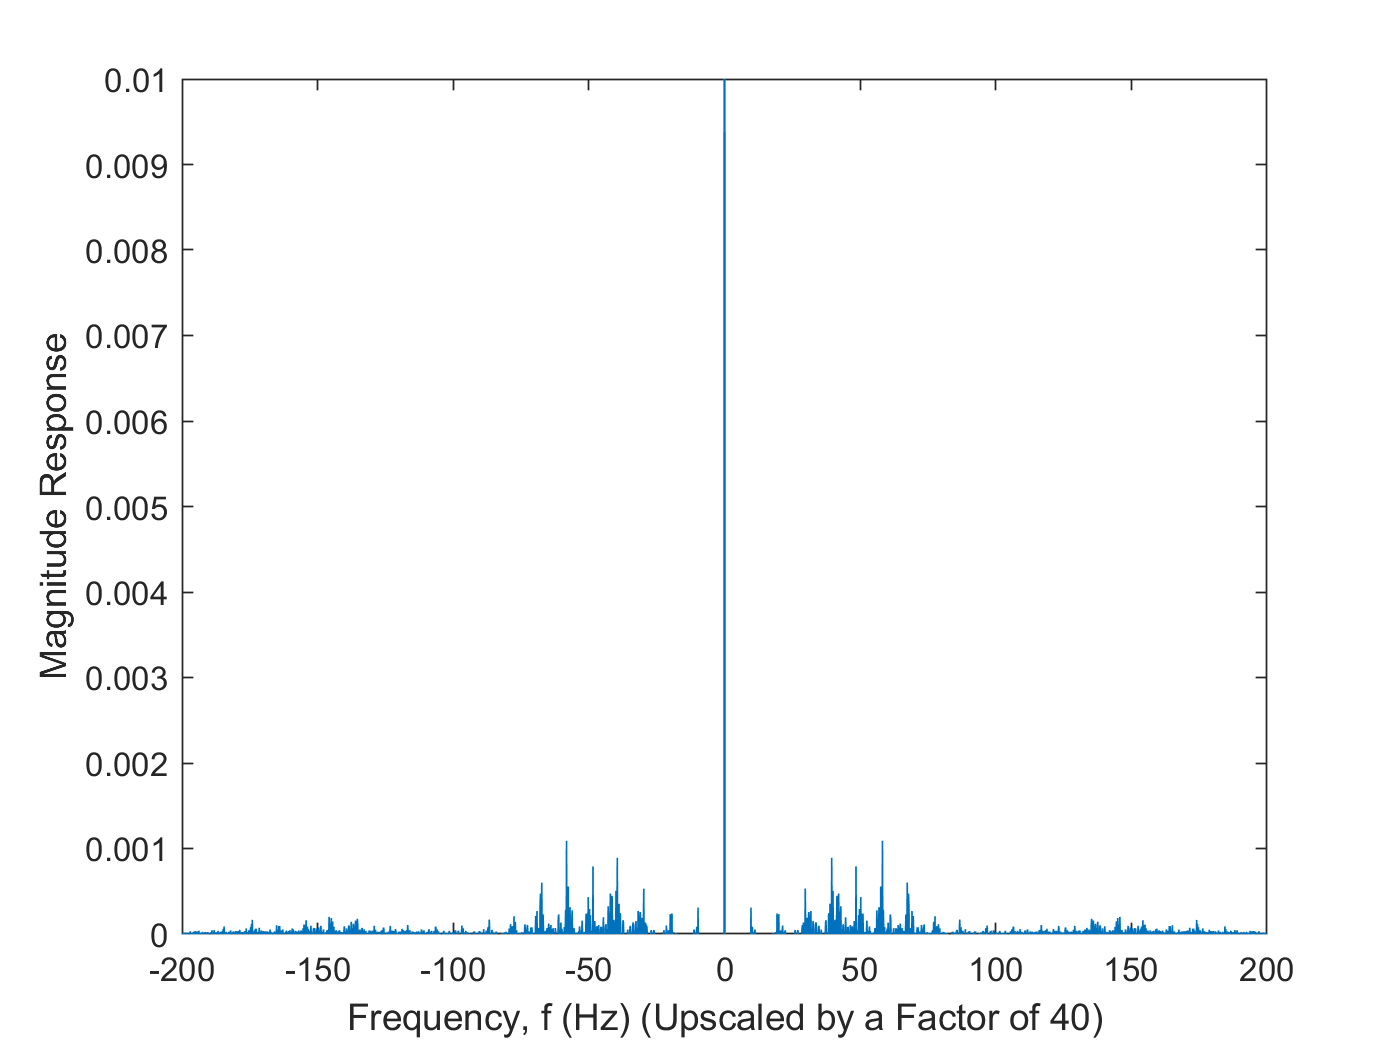
\includegraphics[width=\columnwidth]{JulietLowPassMagZoomed.png}
    \caption{Magnitude response for 20kHz-carried modulated signal (Juliet) after low-pass step (zoomed)}   
    \label{JulietLowpassZoomed}
\end{figure}

\begin{figure}[!htb]
	\centering
  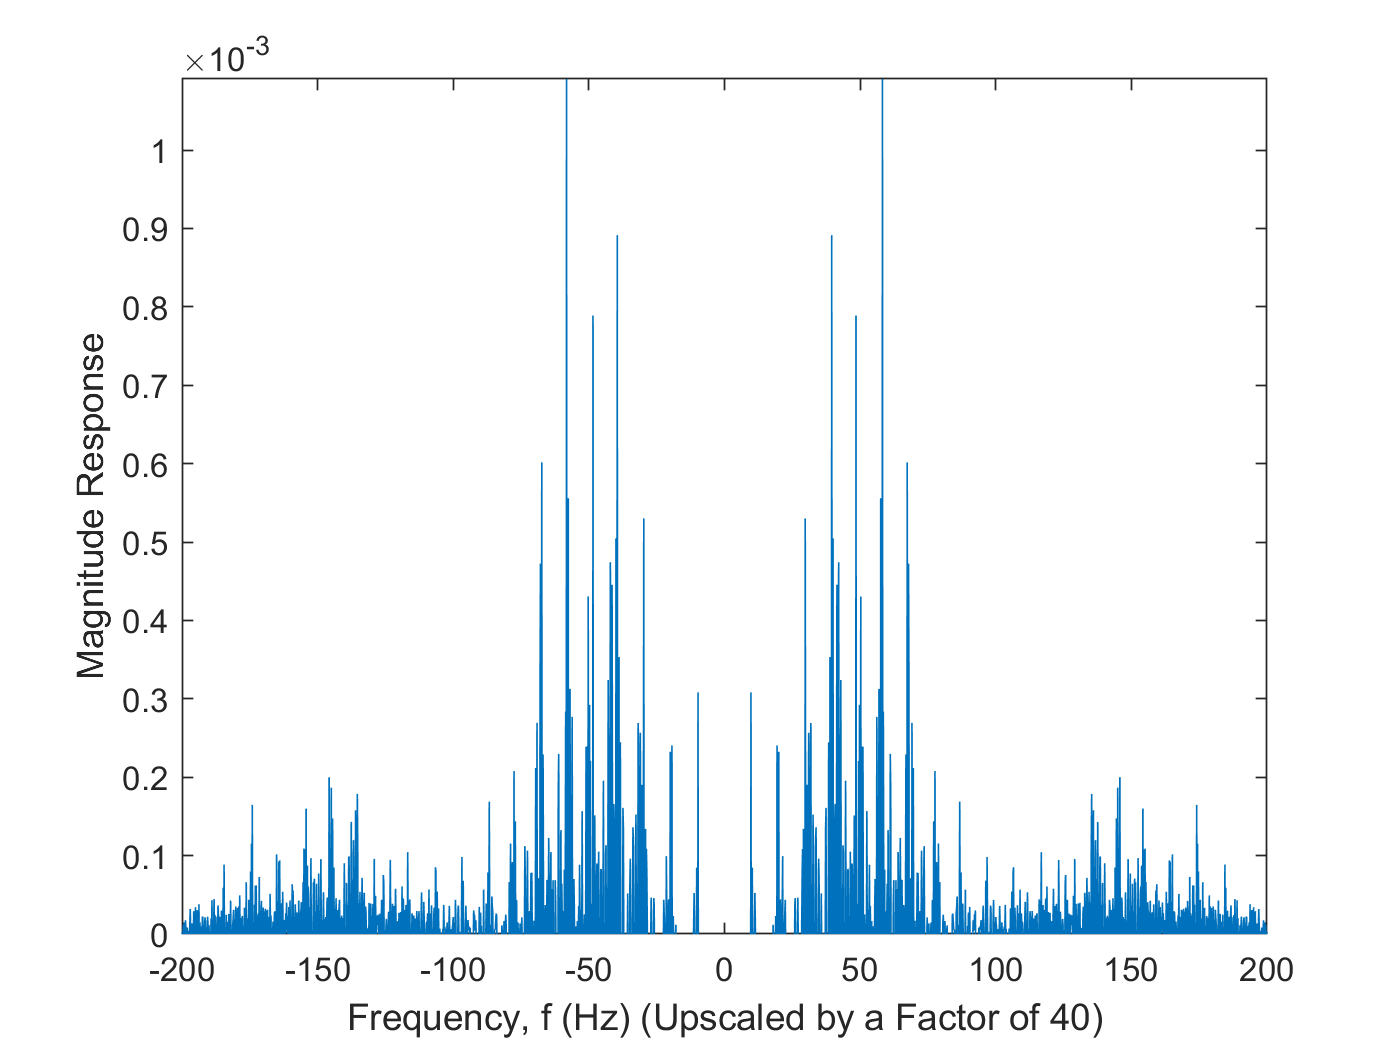
\includegraphics[width=\columnwidth]{JulietMeanRemovedZoomed.png}
    \caption{Magnitude response for 20kHz-carried modulated signal (Juliet) after mean-removal step (zoomed)}   
    \label{JulietMeanRemoved}
\end{figure}

\begin{figure}[!htb]
	\centering
  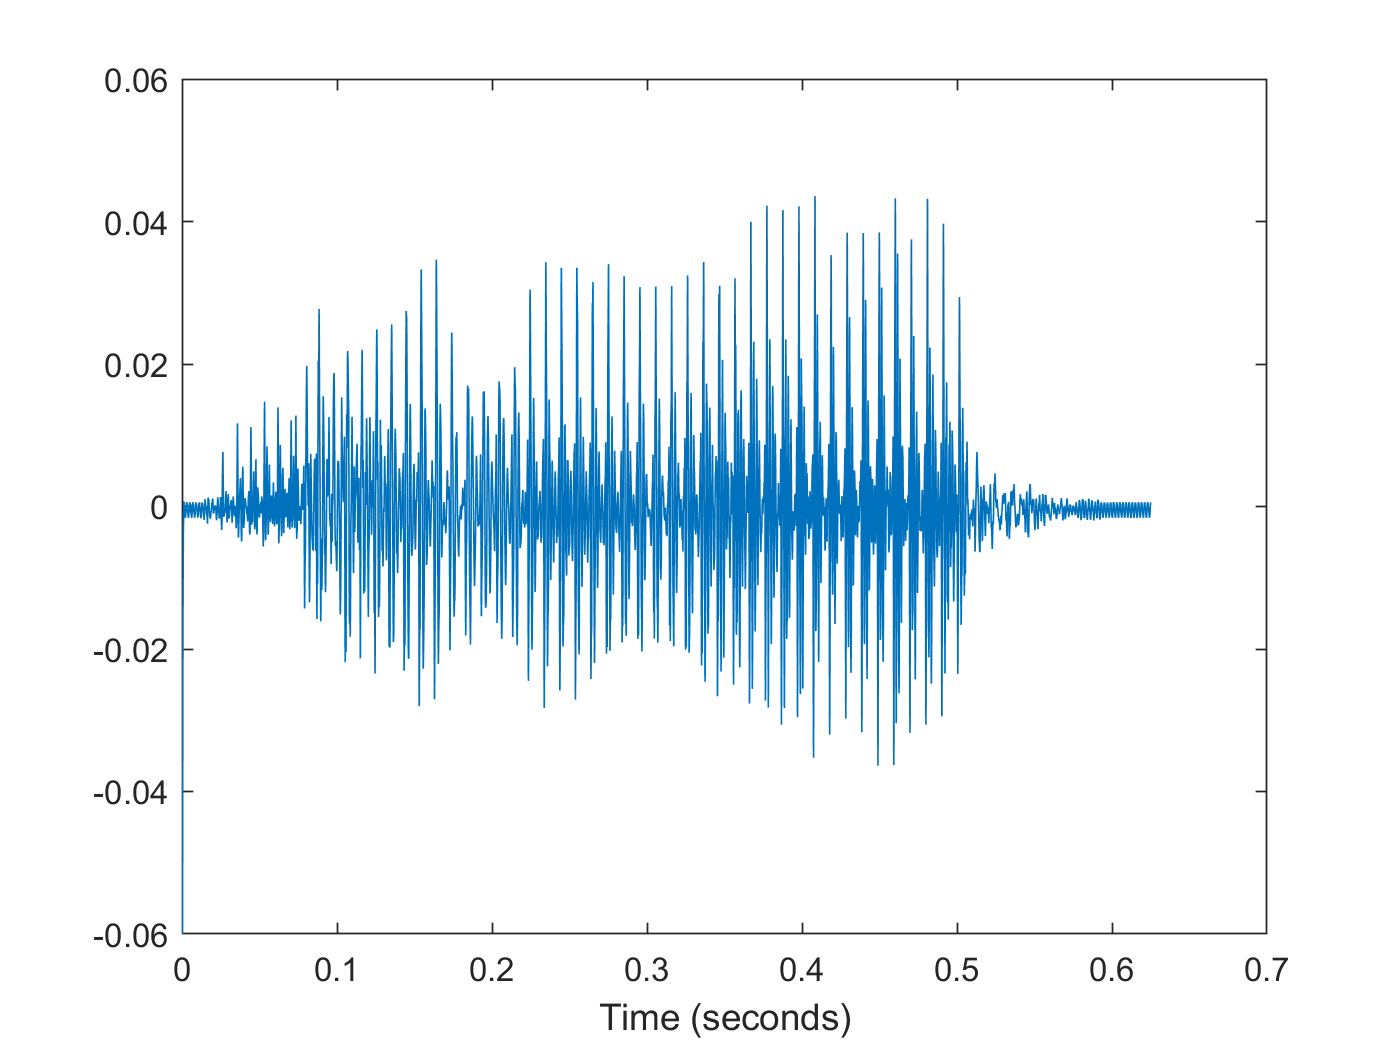
\includegraphics[width=\columnwidth]{JulietTime.png}
    \caption{Magnitude response of the mean-removed, low-passed, rectified, retrieved previously-20kHz-carried signal (Juliet)}   
    \label{JulietTime}
\end{figure}

\subsection{Table of Carrier Signal Frequency and Spoken NATO Phonetic Letter Correspondence}
Our table of which frequencies we found each NATO Phonetic Letter audio sample to be carried by signals of in the provided audio sample is given in Tab. \ref{NATOTable}.

\begin{table}
\centering
\caption{Carrier Frequencies vs NATO Phonetic Letters}
\label{NATOTable}
\begin{tabular}{ll}
NATO Letter & Frequency (kHz) \\
Alfa        & 29              \\
Bravo       & 38              \\
Charlie     & 128             \\
Delta       & 123.5           \\
Echo        & 83              \\
Foxtrot     & 24.5            \\
Golf        & 51.5            \\
Hotel       & 65              \\
India       & 110             \\
Juliet      & 20              \\
Kilo        & 33.5            \\
Lima        & 56              \\
Mike        & 101             \\
November    & 105.5           \\
Oscar       & 92              \\
Papa        & 74              \\
Quebec      & 87.5            \\
Romeo       & 60.5            \\
Sierra      & 114.5           \\
Tango       & 47              \\
Uniform     & 119             \\
Victor      & 42.5            \\
Whiskey     & 78.5            \\
X-Ray       & 96.5            \\
Yankee      & 132.5           \\
Zulu        & 69.5           
\end{tabular}
\end{table}


\section{Conclusion}
In this paper, we have walked through the process of demodulation and gone over some of the mathematics. Additionally, we have demonstrated how to create some of the components that make up a potential demodulator. Finally, we have shown our demodulator in action, deciphering modulated NATO Phonetic Letters from a collection of samples modulated over different frequencies, and overall have provided a guide for those who wish use modulation/demodulation for their own purposes.

\appendices
\section{nth-order Low-Pass Butterworth Filter}
The process for obtaining an nth-order lowpass Butterworth filter with a specified cutoff frequency is demonstrated here.
From \cite{nilsson}, the magnitude response of an nth-order low-pass unity-gain Butterworth filter is given by eq. \eqref{nthordermag}. 
\begin{equation}
\left|H\left(j\omega\right)\right|=\frac{1}{\sqrt{1+\left(\frac{\omega}{\omega_c}\right)^{2n}}}
\label{nthordermag}
\end{equation}
	To form an nth-order unity-gain low-pass Butterworth filter with our given cutoff frequency, therefore, we need a function that a) satisfies this requirement, and b) for which the magnitude response prior to the corner frequency is 1. 
Observe that, for $H(j\omega)$, by complex conjugate multiplication properties \eqref{nthordermag} implies \eqref{nthordersplitomegamag}, which, letting $s=j\omega$, yields eq. \eqref{nthordersplitsmag}.
\begin{equation}
H\left(jw\right)H\left(-jw\right)=\left|H\left(jw\right)\right|^2=\frac{1}{1+\frac{\omega^{2n}}{\omega_c^{2n}}}
\label{nthordersplitomegamag}
\end{equation}
\begin{equation}
H\left.\left(s\right.\right)H\left.\left(-s\right.\right)=\frac{1}{1+\frac{\left(-s^2\right)^n}{\omega_c^{2n}}}=\frac{1}{1+\frac{\left(-1\right)^ns^{2n}}{\omega_c^{2n}}}
\label{nthordersplitsmag}
\end{equation}
	Consequently, we can retrieve a viable $H(s)$ by finding the roots of $1+\frac{\left(-1\right)^ns^{2n}}{\omega_c^{2n}}$ and assigning those that reside in the left-half-plane as factors in the denominator of $H(s)$ (and, by extension, the factors of the right-half-plane as factors in the denominator of $H(-s)$). At this point, all that remains is to scale our current function from its current value to one satisfying the unity gain requirement; we can accomplish this by introducing the constant of the denominator into the numerator. We have designed a Mathematica program to automate this process and attached a PDF of its execution and source code to the end of this document.





% Can use something like this to put references on a page
% by themselves when using endfloat and the captionsoff option.
\ifCLASSOPTIONcaptionsoff
  \newpage
\fi



% trigger a \newpage just before the given reference
% number - used to balance the columns on the last page
% adjust value as needed - may need to be readjusted if
% the document is modified later
%\IEEEtriggeratref{8}
% The "triggered" command can be changed if desired:
%\IEEEtriggercmd{\enlargethispage{-5in}}

% references section

% can use a bibliography generated by BibTeX as a .bbl file
% BibTeX documentation can be easily obtained at:
% http://www.ctan.org/tex-archive/biblio/bibtex/contrib/doc/
% The IEEEtran BibTeX style support page is at:
% http://www.michaelshell.org/tex/ieeetran/bibtex/
%\bibliographystyle{IEEEtran}
% argument is your BibTeX string definitions and bibliography database(s)
%\bibliography{IEEEabrv,../bib/paper}
%
% <OR> manually copy in the resultant .bbl file
% set second argument of \begin to the number of references
% (used to reserve space for the reference number labels box)
\begin{thebibliography}{1}

\bibitem{grant}
J.~Grant, “Experiments and Results in Wireless Telephony,” The American 	Telephone Journal, vol. 15, no. 4, pp. 68–80, Jan. 1907.
\bibitem{white}
J. A. White, Ed., “A Newspaper's Use of the Radio Phone,” The Wireless Age, vol. 8, pp. 10–11, 1920.
\bibitem{nilsson}
J.~Nilsson and S.~Riedel, \emph{Electric Circuits}, 10th~ed.\hskip 1em plus
  0.5em minus 0.4em\relax Boston, United States: Prentice Hall, 2015.

\end{thebibliography}

% biography section
% 
% If you have an EPS/PDF photo (graphicx package needed) extra braces are
% needed around the contents of the optional argument to biography to prevent
% the LaTeX parser from getting confused when it sees the complicated
% \includegraphics command within an optional argument. (You could create
% your own custom macro containing the \includegraphics command to make things
% simpler here.)
%\begin{biography}[{\includegraphics[width=1in,height=1.25in,clip,keepaspectratio]{mshell}}]{Michael Shell}
% or if you just want to reserve a space for a photo:

%\begin{IEEEbiography}[{\includegraphics[width=1in,height=1.25in,clip,keepaspectratio]{picture}}]{John Doe}
%\blindtext
%\end{IEEEbiography}

% You can push biographies down or up by placing
% a \vfill before or after them. The appropriate
% use of \vfill depends on what kind of text is
% on the last page and whether or not the columns
% are being equalized.

%\vfill

% Can be used to pull up biographies so that the bottom of the last one
% is flush with the other column.
%\enlargethispage{-5in}



% that's all folks
\end{document}


%%*************************************************************************
%% Legal Notice:
%% This code is offered as-is without any warranty either expressed or
%% implied; without even the implied warranty of MERCHANTABILITY or
%% FITNESS FOR A PARTICULAR PURPOSE! 
%% User assumes all risk.
%% In no event shall IEEE or any contributor to this code be liable for
%% any damages or losses, including, but not limited to, incidental,
%% consequential, or any other damages, resulting from the use or misuse
%% of any information contained here.
%%
%% All comments are the opinions of their respective authors and are not
%% necessarily endorsed by the IEEE.
%%
%% This work is distributed under the LaTeX Project Public License (LPPL)
%% ( http://www.latex-project.org/ ) version 1.3, and may be freely used,
%% distributed and modified. A copy of the LPPL, version 1.3, is included
%% in the base LaTeX documentation of all distributions of LaTeX released
%% 2003/12/01 or later.
%% Retain all contribution notices and credits.
%% ** Modified files should be clearly indicated as such, including  **
%% ** renaming them and changing author support contact information. **
%%
%% File list of work: IEEEtran.cls, IEEEtran_HOWTO.pdf, bare_adv.tex,
%%                    bare_conf.tex, bare_jrnl.tex, bare_jrnl_compsoc.tex
%%*************************************************************************
